\documentclass[UTF8,a4paper]{ctexart}
\usepackage[margin=1in]{geometry}
\usepackage{fancyhdr,hyperref,float , graphicx}
\pagestyle{fancy}
\hypersetup{hidelinks}

\lhead{\bfseries \leftmark}
\chead{}
\rhead{SCUT}
\lfoot{\url{https://github.com/285571052}}
\cfoot{qhy}
\rfoot{\thepage}
\setlength{\headheight}{13pt}
\renewcommand{\headrulewidth}{0.4pt}
\renewcommand{\footrulewidth}{0.4pt}

\setlength{\parindent}{0pt}
\newcommand{\spaceline}{\vspace{\baselineskip}}

\author{ qhy }
\date{\today}
\title{人工智能}

\begin{document}
\maketitle
\tableofcontents
\newpage

\section{介绍}

\subsection{什么是人工智能?}
人工智能 Artificial Intelligence , 简称 AI , 起源于 美国 1956年的一次夏季讨论(达特茅斯会议)

\begin{itemize}
	\item \textbf{智能机器} : 能够在各类环境中自主地或交互地执行各种拟人任务的机器
	\item \textbf{人工智能(学科)} : 人工智能(学科)是计算机科学中设计研究、设计和因公智能机器的一个分支。它的近期主要目标在于研究用机器来模仿和执行人脑的默写智力功能, 并开发相关理论和技术
	\item \textbf{人工智能(功能)} : 人工智能(能力)是智能机器所执行的通常与人类智能有关的智能行为 , 如判断、推理、证明、识别、感知、理解、通信、设计、思考、规划、学习和问题求解等思维活动
	\item 人工智能是一种使计算机能够思维(内在机制) . 使机器具有治理的激动人心的新尝试
	\item 人工智能研究如何使计算机做事让人过得更好(机器人三大原则)
	\item 人工智能是一门通过计算过程(实现方法)力图理解和模仿智能行为的学科
\end{itemize}

\textbf{AI的本质问题}:研究如何制造出人造的智能机器或系统,来模拟人来智能活动, 以延伸人们智能的科学

\subsection{人工智能研究方法}

\begin{itemize}
	\item 符号主义 : 又称逻辑主义 、心理学派 或计算机学派 , 其原理主要为物理符号系统(即符号操作系统)假设和有限合理性原理\\
	      认为人工智能起源于数理逻辑 , 符号主义仍是人工智能的 主流派

	\item 联结主义 : 又称仿生学派 或 生理学派 , 其原理主要为神经网络及神经网络间的连接机制与学习算法\\
	      认为人工智能源于仿生学 , 特别是人脑模型的研究
	\item 行为主义 : 又称进化主义 或 控制论学派 , 其原理为控制论及感知和行动\\
	      认为人工智能源于控制论 , 这一学派的代表作首推 布鲁克斯的六足行走机器人 ,它被看做新一代的控制论动物, 是一个基于感知-动作模式的模拟昆虫行为的控制系统
\end{itemize}

\textbf{AI的发展历史}
\begin{itemize}
	\item 第一阶段(40-50年代末) 神经元网络时代\\
	      双层网络 , M-P模型 、感知器模型 , 但是 XOR问题不能解决
	\item 第二阶段(50年代中 - 60年代中) , 通用方法时代\\
	      物理符号系统 , 主要研究的问题为 : GPS , 游戏 ,翻译等\\
	      对问题的难度估计不足 ,陷入困境
	\item 第三阶段(60年代中 - 80年代初) , 知识工程时代 \\
	      专家系统 , 知识工程 \\
	      各国发展计划 : 美国星球大战计划 , 日本五代机计划 , 中国865计划
	\item 第四阶段(80年代中 - 90年代初) , 新神经元网络时代 \\
	      BP网络 : 解决了多层学习的问题 \\
	      Hopfield网, 成功求解了旅行商问题\\
	      存在的问题 : 理论依据 , 解决大规模问题的能力\\
	      新的动向 : 构造化方法 / 深度学习
	\item 第五阶段 (90年代初 - 现在) , 海量数据处理与网络时代 \\
	      网络带给AI无限的机会 ,知识发现与数据挖掘 , AI走向实用化, 深度学习 , 稀疏编码
\end{itemize}

知识就是力量 -- 培根

知识蕴含着力量 -- 费根鲍姆

\subsection{人工智能的一些成功}

\begin{itemize}
	\item 1962年 , 证明 $<$数学原理$>$ 书上的全部52个定理
	\item 1976年6月 , 哈肯 , 四色定理证明
	\item 通用问题求解器 GPS
	\item 专家系统
\end{itemize}


\subsection{历史上的人工智能大师}
\begin{itemize}
	\item 阿伦图灵 : 计算机科学理论的创始人\\
	      1912年出生于英国伦敦,1954年去世\\
	      1936年发表论文“论可计算数及其在判定问题中的应用”,提出图灵机理论\\
	      1950年发表论文“计算机与智能”,阐述了计算机可以具有智能的想法,提出图灵测试\\
	      1966年为纪念图灵的杰出贡献,ACM设立图灵奖

	\item 马文 明斯基 , 人工智能之父\\
	      1956年达特茅斯会议的发起人之一\\
	      1958年在MIT创建世界上第一个AI实验室\\
	      1969年获得图灵奖\\
	      1975年首创框架理论
	\item 约翰•麦卡锡 , 人工智能之父\\
	      1956年发起达特茅斯会议,并提出“人工智能”的概念

	      1958年与明斯基一起创建世界上第一个人工智能实验室

	      发明α-β剪枝算法

	      1959年开发LISP语言

	      开创逻辑程序研究,用于程序验证和自动程序设计

	      1971年获得图灵奖

	\item 赫伯特•西蒙 , 符号主义学派的创始人 \\
	      符号主义学派的创始人

	      1916年出生于美国的威斯康辛州


	      1943年在匹兹堡大学获政治学博士学位

	      1969年因心理学方面的贡献获得杰出科学贡献奖

	      1975年和他的学生艾伦•纽厄尔共同获得图灵奖

	      1978年获得诺贝尔经济学奖

	      1986年因行为学方面的成就获得美国全国科学家奖章


	\item 爱德华•费根鲍姆 , 知识工程的提出者 ,	大型人工智能系统的开拓者\\
	      开设Teknowledge和IntelliGenetics两个公司,是世界上第一家以开发和将专家系统商品化的公司
\end{itemize}

\subsection{人工智能应用领域}

人工智能研究及应用领域很多,主要研究领域包括问题求解、机器学习、专家系统、模式识别、自动定理证明、自然语言理解等。

\begin{itemize}
	\item 问题求解 : 人工智能的第一个大成就是发展了能够求解难题的下棋(如国际象棋)程序,它包含问题的表示、分解、搜索与归约等。
	\item 机器学习 : 学习是人类智能的主要标志和获得知识的基本手段;机器学习(自动获取新的事实及新的推理算法)是使计算机具有智能的根本途径;机器学习还有助于发现人类学习的机理和揭示人脑的奥秘。学习是一个有特定目的的知识获取过程,其内部表现为新知识结构的不断建立和修改,而外部表现为性能的改善。
	\item 专家系统 : 一般地说,专家系统是一个智能计算机程序系统,其内部具有大量专家水平的某个领域知识与经验,能够利用人类专家的知识和解决问题的方法来解决该领域的问题。

	      发展专家系统的关键是表达和运用专家知识,即来自人类专家的并已被证明对解决有关领域内的典型问题是有用的事实和过程
	\item 模式识别 : 人工智能所研究的模式识别是指用计算机代替人类或帮助人类感知模式,是对人类感知外界功能的模拟,研究的是计算机模式识别系统,也就是使一个计算机系统具有模拟人类通过感官接受外界信息、识别和理解周围环境的感知能力。
	\item 自动定理证明 : 自动定理证明的研究在人工智能方法的发展中曾经产生过重要的影响。例如,采用谓词逻辑语言的演绎过程的形式化有助于更清楚地理解推理的某些子命题。许多非形式的工作,包括医疗诊断和信息检索都可以和定理证明问题一样加以形式化。因此,在人工智能方法的研究中定理证明是一个极其重要的论题。

	      我国人工智能大师吴文俊院士提出并实现了几何定理机器证明的方法,被国际上承认为“吴氏方法”,是定理证明的又一标志性成果。
	\item 自动程序设计 : 对自动程序设计的研究不仅可以促进半自动软件开发系统的发展,而且也使通过修正自身数码进行学习(即修正它们的性能)的人工智能系统得到发展。程序理论方面的有关研究工作对人工智能的所有研究工作都是很重要的。

	      自动程序设计研究的重大贡献之一是作为问题求解策略的调整概念。已经发现,对程序设计或机器人控制问题,先产生一个不费事的有错误的解,然后再修改它(使它正确工作),这种做法一般要比坚持要求第一个解就完全没有缺陷的做法有效得多。

	\item 自然语言理解 : 语言处理也是人工智能的早期研究领域之一,并引起了进一步的重视。语言的生成和理解是一个极为复杂的编码和解码问题。
	      一个能理解自然语言信息的计算机系统看起来就像一个人一样需要有上下文知识以及根据这些上下文知识和信息用信息发生器进行推理的过程。理解口头的和书写语言的计算机系统所取得的某些进展,其基础就是有关表示上下文知识结构的某些人工智能思想以及根据这些知识进行推理的某些技术。

	\item 机器人学 : 人工智能研究日益受到重视的另一个分支是机器人学,其中包括对操作机器人装置程序的研究。这个领域所研究的问题,从机器人手臂的最佳移动到实现机器人目标的动作序列的规划方法,无所不包。目前已经建立了一些比较复杂的机器人系统。
	      机器人和机器人学的研究促进了许多人工智能思想的发展。
	      智能机器人的研究和应用体现出广泛的学科交叉,涉及众多的课题,机器人已在各领域获得越来越普遍的应用。

	\item 人工神经网络 : 人工神经网络处理直觉和形象思维信息具有比传统处理方式好得多的效果。
	      人工神经网络已在模式识别、图象处理、组合优化、自动控制、信息处理、机器人学和人工智能的其它领域获得日益广泛的应用。

	\item 智能检索 : 随着科学技术的迅速发展,出现了“知识爆炸”的情况,研究智能检索系统已成为科技持续快速发展的重要保证。
	      智能信息检索系统的设计者们将面临以下几个问题。首先,建立一个能够理解以自然语言陈述的询问系统本身就存在不少问题。其次,即使能够通过规定某些机器能够理解的形式化询问语句来回避语言理解问题,但仍然存在一个如何根据存储的事实演绎出答案的问题。第三,理解询问和演绎答案所需要的知识都可能超出该学科领域数据库所表示的知识。

\end{itemize}

\subsection{机器所不能理解的问题}
\begin{itemize}
	\item 视觉游戏--“比泽尔德幻觉”
	      \begin{figure}[H]
		      \centering
		      
\includegraphics[scale = 0.3]{assets/ArtificialIntelligence_9520f.png}
	      \end{figure}
	      比泽尔德幻觉:图中所有的红色看起来都一样吗?
	      【解析】语境会影响你对颜色的感知。所有的红色都是完全一样的。这就是比泽尔德幻觉。

	\item 视觉游戏--“盒子幻觉”
	      \begin{figure}[H]
		      \centering
		      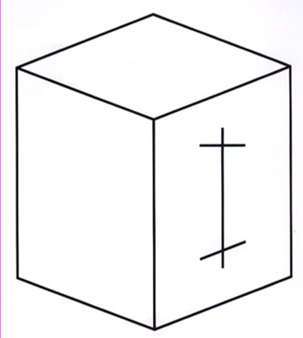
\includegraphics[scale = 0.3]{assets/ArtificialIntelligence_30a23.png}
	      \end{figure}
	      盒子幻觉:看立方体外侧面上的这个图形。哪条线与竖线垂直?哪条线不与竖线垂直?把立方体的边线遮住,你将发现你的感知发生了变化。
	      【解析】盒子幻觉的感知提示为你确定图中心线段的位置提供了一个背景。离开盒子你的视觉系统就必须使用其他背景。这就是盒子幻觉。
	\item ...
\end{itemize}



机器人学三大法则 -- 电影 : 我 、 机器人
\begin{itemize}
	\item 一.机器人不得伤害人,也不得见人受到伤害而袖手旁观
	\item 二.机器人应服从人的一切命令,但不得违反第一定律
	\item 三.机器人应保护自身的安全,但不得违反第一、第二定律
\end{itemize}

\section{搜索问题}
许多问题 , 都可以归结为 在某一状态空间中搜索目标或路径的问题

比如 : 汉诺塔问题 、 8数码问题 、 迷宫问题 、农夫过河问题 、装箱与布局问题 、 排班问题等

\subsection{状态空间法}

\textbf{对于非结构化问题,即不能使用数学来进行描述的问题,我们怎么使用计算机进行描述?}\\
使用\textbf{状态空间法:}
\begin{itemize}
	\item 使用多元组来描述问题的状态
	\item 每个问题有初始态和目标抬
	\item 有些状态是非法的
	\item 我们需要做的是,从初始态转移到目标态
\end{itemize}

\begin{figure}[H]
	\centering
	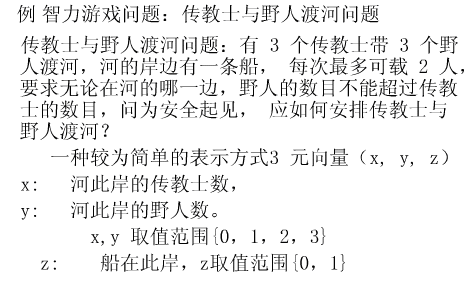
\includegraphics[scale = 0.6]{assets/ArtificialIntelligence_8e77e.png}
	\caption{传教士与野人渡河问题 - 表示}
\end{figure}

\begin{figure}[H]
	\centering
	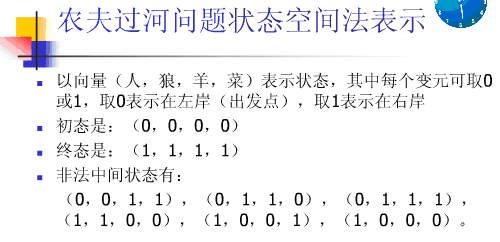
\includegraphics[scale = 0.6]{assets/ArtificialIntelligence_e824b.png}
	\caption{农夫过河问题 - 表示}
\end{figure}

基本过程 :
\begin{itemize}
	\item 为问题选择适当的状态和操作的形式化描述
	\item 从某个初始状态出发 ,每次使用一个操作 ,递增地建立操作序列 , 直到达到目标状态为止
\end{itemize}

状态空间的搜索方式:
\begin{itemize}
	\item 盲目搜索
	\item 启发式搜索
\end{itemize}

\subsection{回溯搜索}

回溯搜索:不断扩展路径,直到终点或死路\\
存在的问题:
\begin{itemize}
	\item 深度问题\\
	      搜索的深度过深(出现爆栈等问题)\\
	      解决办法:对深度加以限制
	\item 死循环问题\\
	      寻路过程可能陷入循环之中\\
	      解决办法:记录从初始状态到当前状态的路径(图搜索)
\end{itemize}

\subsection{图搜索}

回溯搜索:只保留从初始状态到当前状态的一条路径\\
图搜索:保留所有已经搜索过的路径

具体地看, 回溯搜索只管不断回溯和搜索 而不进行必要的判断 ,而图搜索则是会进行必要的条件判断,比如已经到过的状态(阶段)不会继续扩展

在图搜索中 ,对于已经搜索过的状态(节点) , 会从OPEN表\footnote{OPEN表存放待扩展的节点 , 初始为根节点}中移除 ,而放入 CLOSED 表\footnote{CLOSED表存放已经扩展过的节点}

\subsubsection{无信息图搜索过程}
\begin{itemize}
	\item dfs\\
	      不保证有解\\
	      深度限制不合理,可能找不到解(可以将算法改为可变深度限制,比如迭代加深?)\\
	      最坏情况等于穷举\\
	\item bfs\\
	      当图有解时,一定能找到最优解\\
	      效率低
\end{itemize}
两者的区别是对于OPEN表中节点的扩展顺序 ,dfs优先扩展深度大的节点 ,而bfs则优先扩展深度小的节点

\subsubsection{启发式图搜索}
启发式图搜索:引入启发知识,希望在保证找到最佳解的情况,尽可能减少搜索范围,提高搜索效率(引入强的知识 ,可能找不到最优解)\\

定义一个评价函数f,对当前搜搜状态进行评估,找出最有希望的节点来扩展

\subsection{A算法}
启发式搜索算法A, 简称A算法

A算法:$f(n) = g(n) + h(n)$\\
其中,$f(n)$为评价函数,$h(n)$为启发函数 , $g(n)$为当前开销

定义$g^*(n)$为从s到n的最短路径的耗散值,$h^*(n)$为从n到g的最短路径的耗散值,$f^*(n) = g^*(n) + h^*(n)$为从s经过n到g的最短路径的耗散值\\
$g(n) , h(n) , f(n)$是对三者的估计

A算法的过程 : 按f(n)递增的顺序来排列OPEN表中的节点 , 优先扩展 f(n)小的节点

\textbf{A算法例子}:
\begin{figure}[H]
	\centering
	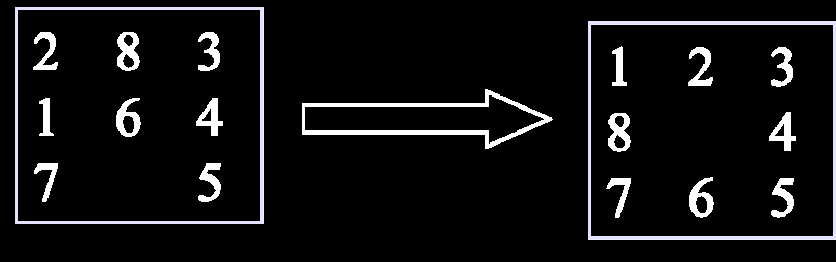
\includegraphics[scale = 0.3]{assets/ArtificialIntelligence_2e222.png}
\end{figure}

定义评价函数 : $f(n) = g(n) + h(n)$\\
$g(n)$:从初始节点到当前节点的耗散值\\
$h(n)$ :当前节点的"不在位"的将牌数

\subsection{爬山法}

爬山法(局部搜索算法):$f(n) = h(n)$(只考虑还需要的最少耗散)

\subsection{分支限界法}

分支限界法:如果对于任何的n,$f(n) = g(n) , h(n) = 0$(只考虑当前的最少耗散)

\subsection{动态规划法}

动态规划算法:当$h(n) = 0$时,对于某个中间节点l,只考虑,s到l的最短路径分支,而不考虑其他

\subsection{A*算法}

最佳图搜索算法:A*算法,在A算法中,如果满足$h(n) \leq h^*(n)$,则称A算法为A*算法(也就是放宽了约束条件)

\textbf{A*算法的假设}:
设$n_i$、$n_j$是任意两个节点 , 有 $C(n_i , n_j) > \epsilon$ , 其中 $\epsilon$ 为大于 0 的常数

几个等式 :$f^*(s) = f^*(t) = h^*(s) = g^*(t) = f^*(n)$\\
,其中s是初始节点 , t是目标节点 , n是s到t的最佳路径上的节点

\begin{itemize}
	\item \textbf{定理1:}对有限图 , 如果从初始节点s到目标节点有路径存在 ,则算法A一定成功结束
	\item \textbf{引理1:}对于无限图,若有从初始节点s到目标节点t的路径 ,则$A^*$不结束时 , 在OPEN表中即使最小的f值也将增到任意大, 或有$f(n) > f^*(n)$
	\item \textbf{引理2:}$A^*$结束前 , OPEN表中必存在$f(n)\leq f^*(s)$, n在最佳路径上\\
	      存在一个节点 n , n在最佳路径上 $f(n) = g(n) + h(n) = g^*(n) + h(n) \leq g^*(n) + h^*(n) = f^*(n) = f^*(s)$
	\item \textbf{定理2:} 对无限图 , 若从初始节点s到目标节点t有路径存在 ,则$A^*$算法一定成功结束。

	      引理1:$A^*$如果不结束 ,则OPEN中所有的n有$f(n) > f^*(s)$

	      引理2:在$A^*$结束前 , 必存在节点n , 使得 $f(n) \leq f^*(s)$

	      如果存在$A^*$不结束 , 将导致矛盾
	\item \textbf{定理3:}(可采纳性定理)若存在从初始节点s到目标节点t的路径 ,则$A^*$必能找到最佳解结束

	      由定理1,2知 , $A^*$一定找到一条路径结束 \\
	      设找到的路径$s\to t$不是最佳的(t为目标) , 则$f(t) = g(t) > f^*(s)$

	      由引理2知,结束前OPEN中存在$f(n) \leq f^*(s)$的节点n , 所以$f(n) \leq f^*(s) < f(t)$

	      因此$A^*$应选择n扩展,而不是t。与假设$A^*$选择t结束 ,矛盾 ,得证

	\item \textbf{推论2:}$A^*$选作扩展的任意节点 , $f(n) \leq f^*(s)$

	      由引理2知 , 在$A^*$结束前 , OPEN中存在节点$n'$ , $f(n') \leq f^*(s)$

	      设此时$A^*$选择n扩展 , 如果$n = n'$ , 则$f(n) \leq f^*(s)$得证

	      如果$n\neq n'$ , 由于 $A^*$选择n扩展 ,而不是 $n'$ , 所以有
	      $f(n) \leq f(n') \leq f^*(s)$ , 得证

	\item \textbf{定理4:} 设对同一个问题定义了两个$A^*$算法 $A_1
	      $和 $A_2$ , 若$A_2$ 比 $A_1$有较多的启发信息 , 即对所有非目标节点有$h_2(n) > h_1(n)$ , 则在具有一条从s到t的路径的隐含图上 ,搜索结束时, 由$A_2$所扩展的每个节点 , 也必定 由 $A_1$ 所扩展 , 即$A_1$扩展的节点数至少和$A_2$一样多

	      简写: 如果$h_2(n) > h_(n)$(目标节点除外) , 则$A_1$扩展的节点数$\geq$ $A_2$扩展的节点数

	      使用数学归纳法,对节点深度进行归纳 :

	      当$d(n) = 0$时, 即只有一个节点 ,显然定理成立

	      设$d(n) \leq k$时,定理成立(归纳假设)

	      当$d(n) = k + 1$时 , 用反证法 :

	      设存在一个深度为k+1的节点n,被$A_2$ 扩展 ,但没有被$A_1$扩展 ,而由假设 , $A_1$扩展了n的父节点 , 即n已经被生成了 ,因此当$A_1$结束时, n将被保留在OPEN表

	      所以有$f_1(n) \geq f^*(s)$ , 即 $g_1(n) + h_1(n) \geq f^*(s)$

	      另一方面 , 由于 $A_2$ 扩展了 n , 有 $f_2(n) \leq f^*(s)$(引理2) , 即$h_2(n) \leq f^*(s) - g_2(n)$

	      由于$d(n) = k$时, $A_2$扩展的节点$A_1$一定扩展 ,有 $g_1(n) \leq g_2(n)$(因为$A_2$的路$A_1$均走到了)

	      所有 : $h_1(n) \geq f^*(s) - g_1(n) \geq f^*(s) - g_2(n)$

	      综上 , 有 $h_1(n) \geq h_2(n)$  , 与定理条件矛盾 ,故得证
\end{itemize}

\textbf{对h的评价方法:}平均分叉数 , 设共扩展了d层节点 ,共搜索了N个节点 , 则
\[N = \frac{1 - b^{*(d + 1)}}{1 - b^*}\]
,其中 , $b^*$称为平均分叉数 , $b^*$越小 , 说明$h$效果越好 , $b^*$是一个稳定的常数 ,同一问题基本不随问题规模变化

A*算法的改进:可能会出现在求最优解的时候多次重复扩展同一个节点的情况,因为扩展的时候,并不是找到从初始节点到当前节点的最短路径(相当于枚举了所有的路径)\{改进之后的,才是我学的那个A*算法,设置上界,不满足上界的不要\}

解决办法:
\begin{itemize}
	\item 对h加以限制,使得第一次扩展一个节点的时候,就找到了从s到当前节点的最短路径\\
	      也就是选择节点的时候,选择到当前节点开销最小的节点
	      \begin{figure}[H]
		      \centering
		      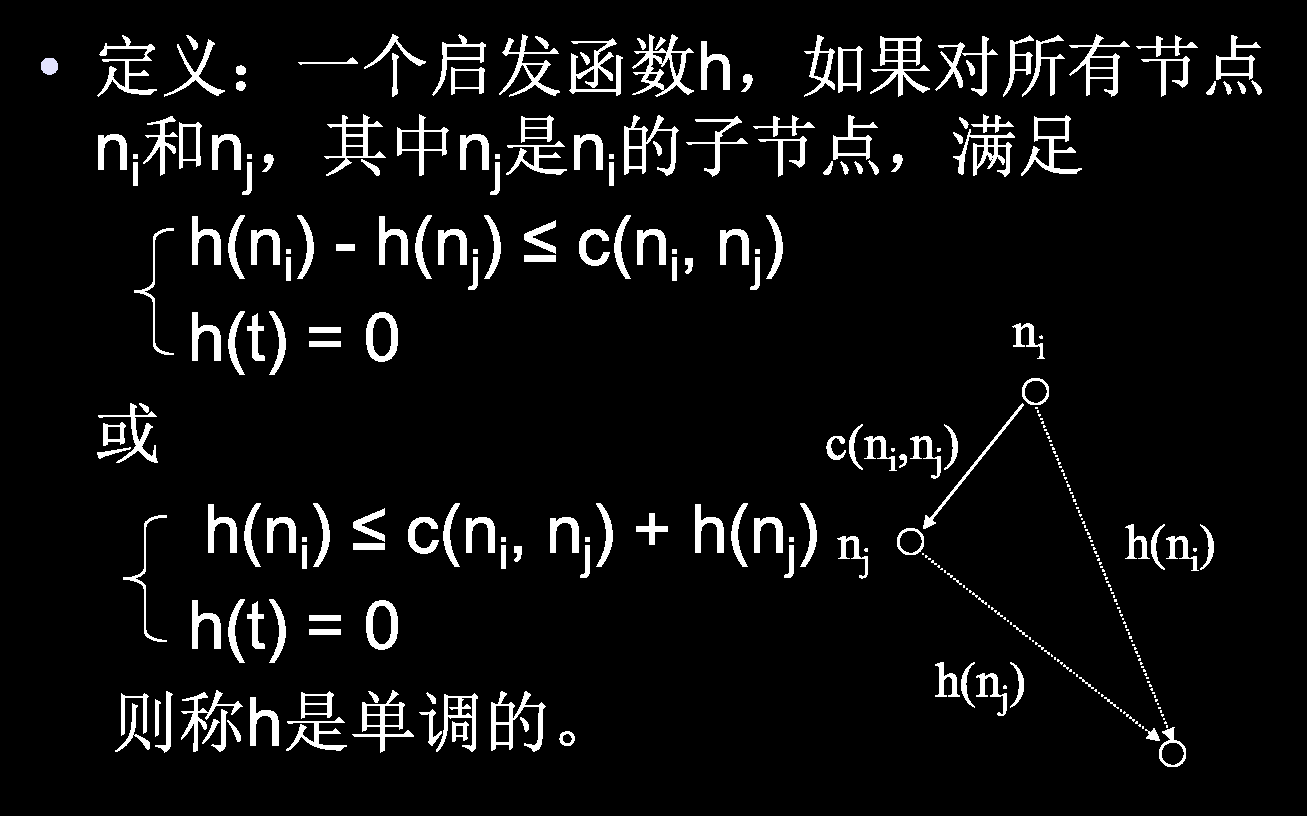
\includegraphics[scale = 0.3]{assets/ArtificialIntelligence_61699.png}
		      \caption{对h增加 单调约束}
	      \end{figure}
	\item 对算法加以改进,改进算法,避免多次扩展\\
	      记录一个预测上界,如果比这个上界还大的节点,不再加入open 表
\end{itemize}

算法讨论 : 盲目搜索算法产生组合爆炸 , 启发搜索算法属于弱方法 ,不能保证找到解

\section{与或图搜索}

% 第二章 与或图搜索问题
与或图搜索问题:有些问题的解不移动是路径,而是子图,节点与其后续节点存在与关系,也存在或关系,这类图称为与或图
即,搜索的过程,不一定走一个分支,可能需要同时满足两个分支都能达到终态

\begin{figure}[H]
	\centering
	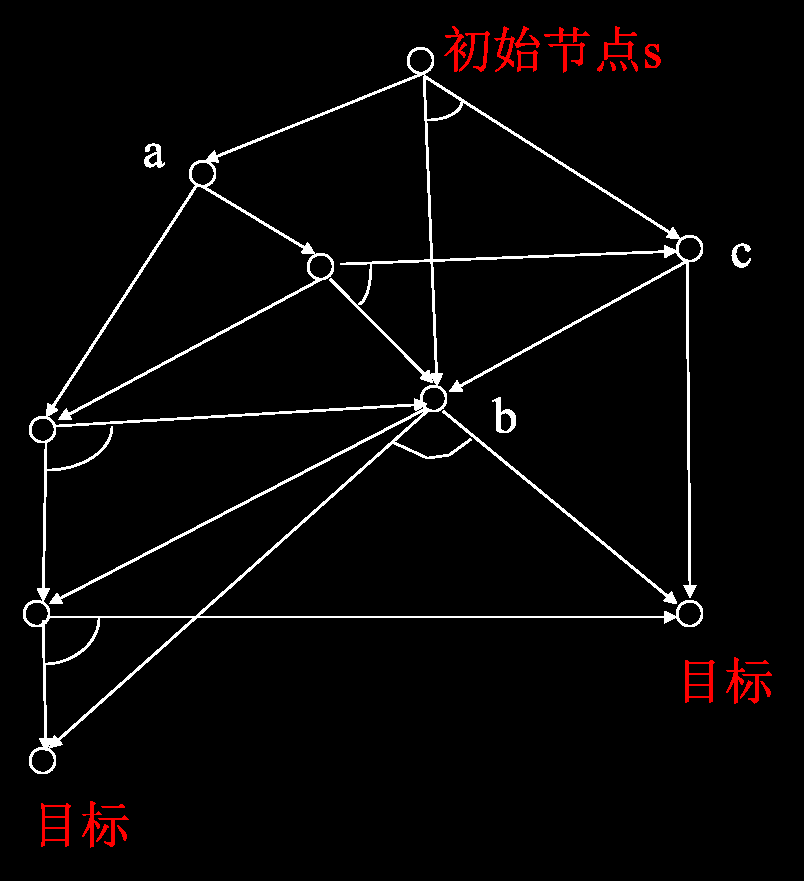
\includegraphics[scale = 0.3]{assets/ArtificialIntelligence_76d7c.png}
	\caption{问题等价变换求解 : 问题分解成子问题进行求解}
\end{figure}

与或图是一个超图, 节点间通过连接符连接:
\begin{figure}[H]
	\centering
	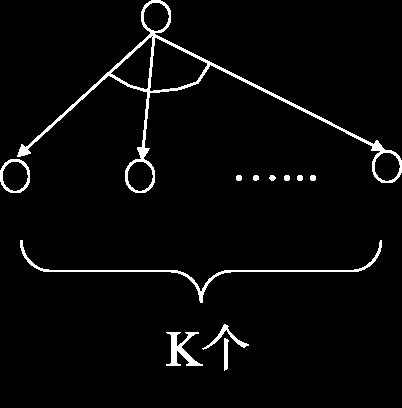
\includegraphics[scale = 0.3]{assets/ArtificialIntelligence_ed995.png}
	\caption{k-连接符:表示k个子问题都要求解完才能解决原始问题}
\end{figure}

耗散值的计算:
\[k(n,N) = C_n + k(n_1 , N) + \cdots + k(n_i , N)\]
其中 , $N$终节点集 , $C_n$为连接符的耗散值

\subsection{与或图搜索$AO^*$算法}
和$A^*$算法类似:
\begin{itemize}
	\item 扩展节点 : 从最优的局部图中选择一个节点扩展
	\item 计算耗散值的过程 : 对当前的局部图重新计算耗散值
\end{itemize}

\begin{figure}[H]
	\centering
	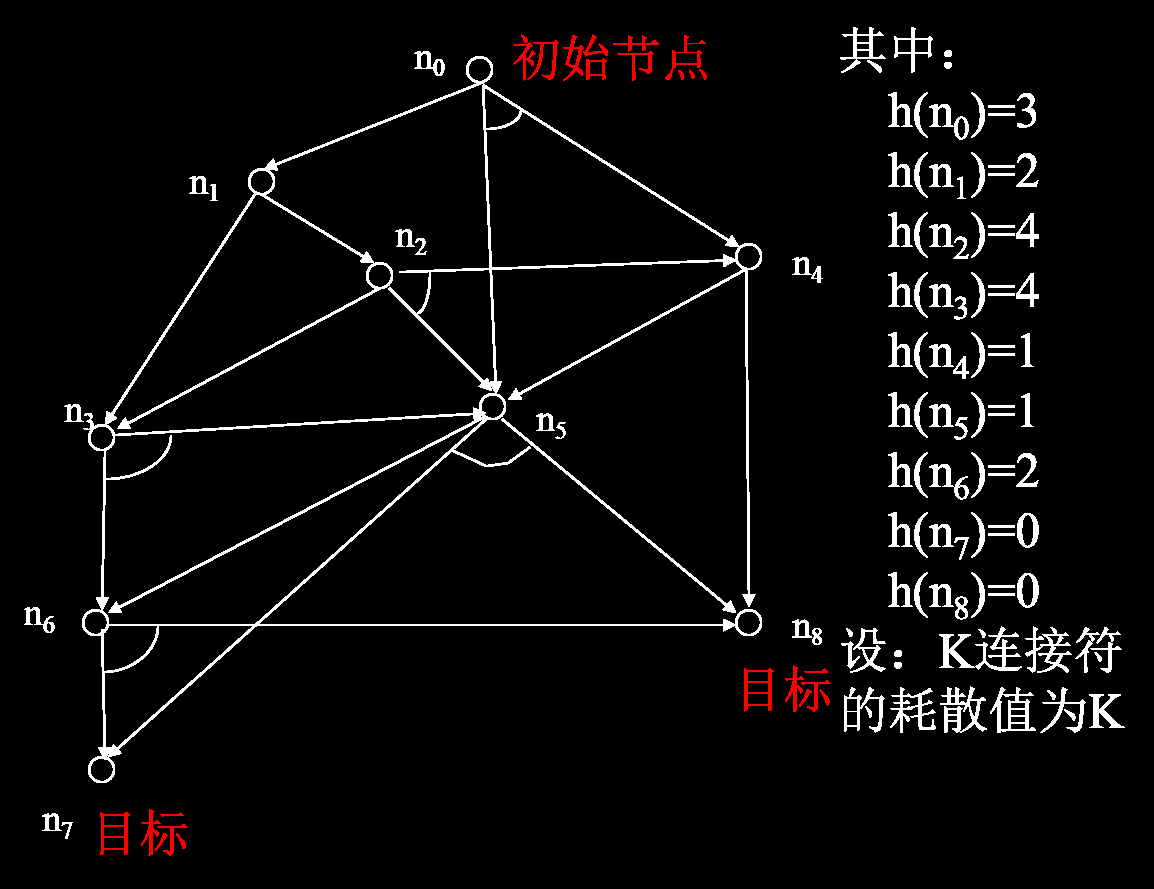
\includegraphics[scale = 0.3]{assets/ArtificialIntelligence_d9a6d.png}
	\caption{$AO^*$算法举例}
\end{figure}

\begin{figure}[H]
	\centering
	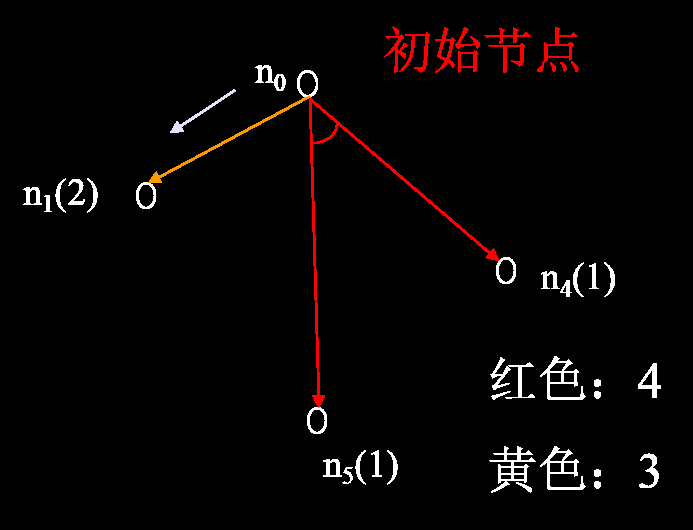
\includegraphics[scale = 0.15]{assets/ArtificialIntelligence_f13c1.png}
	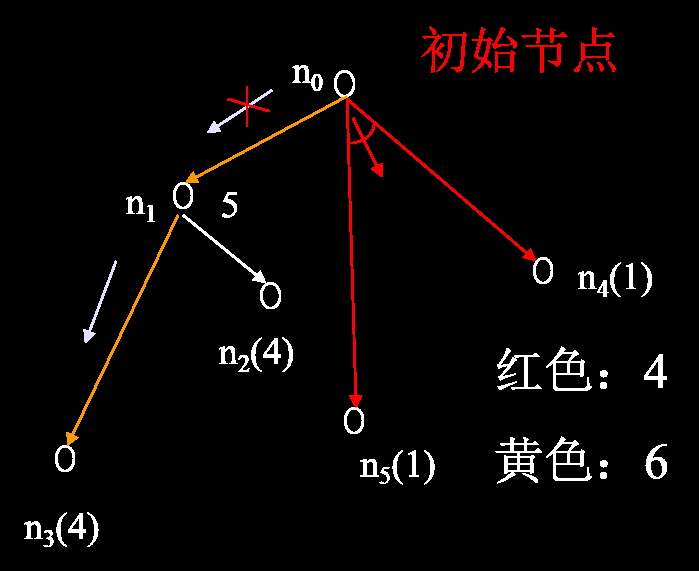
\includegraphics[scale = 0.15]{assets/ArtificialIntelligence_72957.png}
	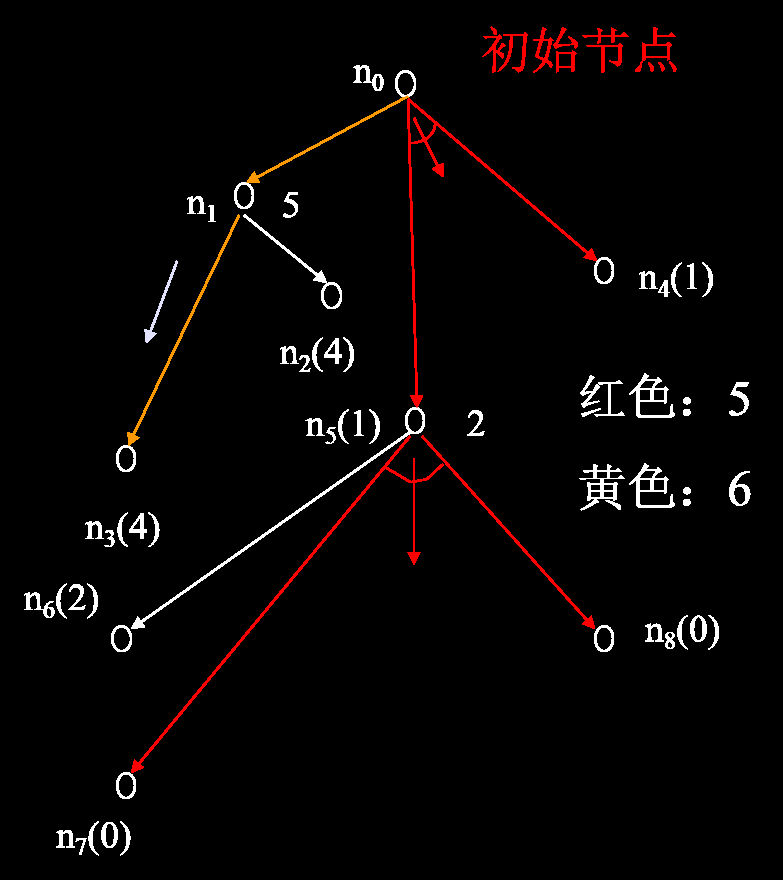
\includegraphics[scale = 0.15]{assets/ArtificialIntelligence_c0b3a.png}
	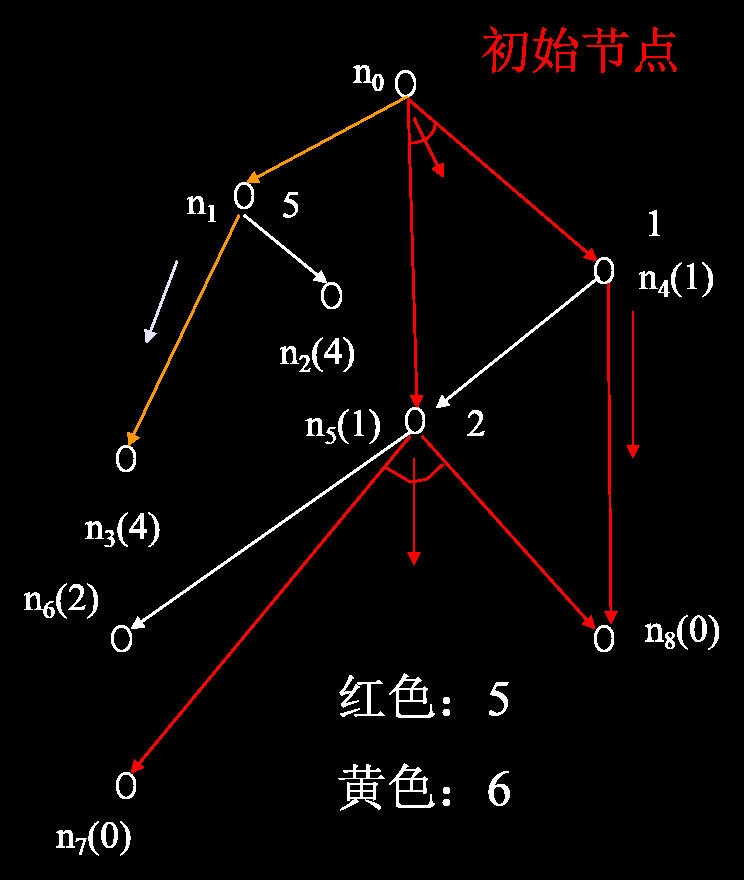
\includegraphics[scale = 0.15]{assets/ArtificialIntelligence_8de7f.png}
	\caption{黄色和红色表示路径的当前开销 , 选择开销小的点扩展 , 注意 , 一条边的 表示 1-连接 , 也要计算开销 1}
\end{figure}

\subsection{博弈树搜索}

博弈问题:
\begin{itemize}
	\item 双人
	\item 一人一步
	\item 双方信息完备
	\item 零和
\end{itemize}

极大极小过程中,棋局评价函数的特点:
\begin{itemize}
	\item 先生成局部格局,再对格局进行评估
	\item 两个过程分开进行
	\item 效率低 :因为要把整棵树完全展开才能计算
\end{itemize}

$\alpha \beta$剪枝:
\begin{itemize}
	\item 极大节点的下界为$\alpha$
	\item 极小节点的上界为$\beta$
	\item 剪枝条件:
	      \begin{itemize}
		      \item $\alpha$剪枝:后辈节点的$\beta$值$\leq$祖先节点的$\alpha$值
		      \item $\beta$剪枝:后辈节点的$\alpha$值$\geq$祖先节点的$\beta$值
	      \end{itemize}
	% \item 简记:
	%       \begin{itemize}
	% 	      \item 极小$\leq$极大
	% 	      \item 极大$\geq$极小
	%       \end{itemize}
\end{itemize}

\section{归结推理方法}

% 第三章 归结推理方法
\textbf{命题:}能判断真假的陈述句。

\textbf{子句集:}合取范式形式下的子命题(元素)的集合

例:命题公式:PΛ( P∨Q)Λ( ~P∨Q)

子句集 S:S = {P, P∨Q, ~P∨Q}

\textbf{归结法:}消除互补对,求新句子,得到归结式(证明命题用)

\textbf{归结过程:}
\begin{itemize}
	\item 将命题写成合取范式
	\item 求出子句集
	\item 对子句集使用归结推理规则
	\item 归结式作为新子句参加归结
	\item 归结式为空子句,S是不可满足的(矛盾),原命题成立。
\end{itemize}

\textbf{谓词归结:}\\
\textbf{前束范式:}一切量词都在公式的最左边(不含否定词),且这些量词的管辖域都延伸到公式的末端\\
\textbf{Skolem标准形}:前束范式消去量词之后的谓词公式

\textbf{求子句集:}
\begin{itemize}
	\item 求前束范式
	\item 求出Skolem标准形 , 消去存在变量 : $\forall x$中$x$的函数 $f(x)$ 代替 $\exists y$
	\item 使用,代替合取符号$\land$,并表示成集合形式
\end{itemize}

\textbf{归结原理:}\\
\textbf{置换:}使用置换项去置换变量\\
例如\\
\{a/x,c/y,f(b)/z\}是一个置换。\\
\{g(y)/x,f(x)/y\}不是一个置换, \\

\begin{figure}[H]
	\centering
	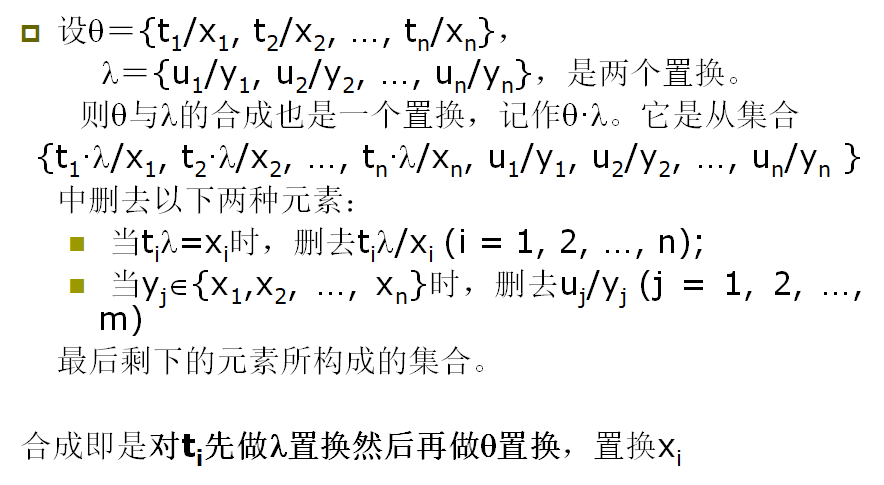
\includegraphics[scale = 0.3]{assets/ArtificialIntelligence_3ac55.png}
	\caption{置换的合成}
\end{figure}

\textbf{合一:}寻找相对变量的置换,使两个谓词公式一致
例:\\
设有公式集F={P(x, y, f(y)), P(a,g(x),z)},则\{a/x, g(a)/y, f(g(a))/z\}是它的一个合一。\\
注意:一般说来,一个公式集的合一不是唯一的。

% 归结过程的策略控制:

% \textbf{Herbrand定理:}
% \begin{itemize}
% 	\item 子句集S是不可满足的,当且仅当对应于S的完全语义数是棵有限封闭树。

% 	\item 子句集S是不可满足的,当且仅当存在不可满足的S的有限基例集。

% \end{itemize}

\section{知识表示}
\subsection{知识}

\textbf{知识种类}
\begin{itemize}
	\item 事实性知识:采用直接表示的形式\\
	      如:凡是猴子都有尾巴
	\item 过程性知识:描述做某件事的过程\\
	      如:电视维修法
	\item 行为性知识:不直接给出事实本身,只给出它在某方面的行为\\
	      如:微分方程、(事物的内涵)
	\item 实例性知识:只给出一些实例,知识藏在实例中。
	\item 类比性知识: 即不给出外延,也不给出内涵,只给出它与其它事物的某些相似之处 \\
	      如:比喻、谜语
	\item 元知识:有关知识的知识。最重要的元知识是如何使用知识的知识,如何从知识库中找到想要的知识。
\end{itemize}

\textbf{知识的要素:}
\begin{itemize}
	\item 事实:事物的分类、属性、事物间关系、科学事实、客观事实等。(最低层的知识)
	\item 规则:事物的行动、动作和联系的因果关系知识。(启发式规则)。
	\item 控制:当有多个动作同时被激活时,选择哪一个动作来执行的知识。(技巧性)
	\item 元知识:高层知识。怎样实用规则、解释规则、校验规则、解释程序结构等知识。
\end{itemize}

\textbf{知识表示的定义:}
\begin{itemize}
	\item 知识表示研究用机器表示知识的可行性、有效性的一般方法。
	\item 知识表示是理智推理的部分理论。
	\item 知识表示是有效计算的载体
	\item 知识表示是交流的媒介(如语义网络)
\end{itemize}

\textbf{选取知识表示的因素}:
\begin{itemize}
	\item 表示范围是否广泛
	\item 是否适于推理
	\item 是否适于计算机处理
	\item 是否有高效的算法
	\item 能否表示不精确知识
	\item 能否模块化
\end{itemize}


\textbf{知识的表示方法:}

\begin{figure}[H]
	\centering
	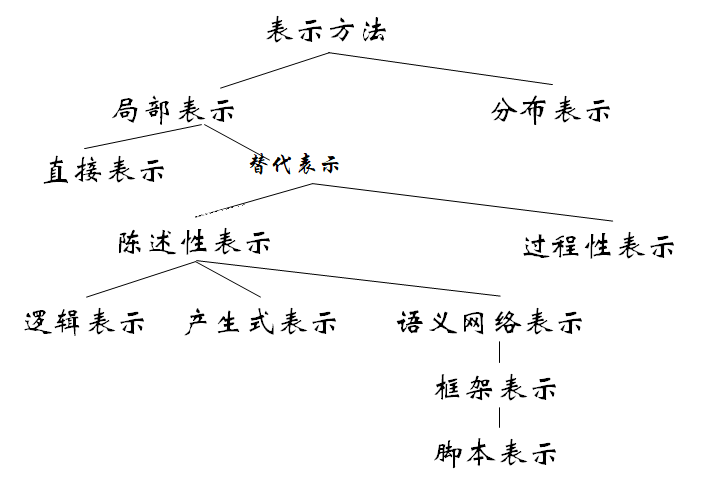
\includegraphics[scale = 0.3]{assets/ArtificialIntelligence_9d3f2.png}
	\caption{表示方法}
\end{figure}

表示方法分类:
\begin{itemize}
	\item 局部表示类 : 最充分也是正统AI最经常使用的
	\item 分布表示法 : 对局部表示法在智能行为表述尚不够而作的补充
\end{itemize}

\textbf{直接表示} : 正在引起越来越多AI研究者的注意。(不可完全独立:考虑到“任何表示方法必须被计算机所接受” 这个先决条件,直接表示需要借助局部或部分表示形式。

\subsection{谓词逻辑法}

\textbf{逻辑表示法} : 谓词逻辑规范表达式:
P ( x1, x2, x3, …), 这里P是谓词, xi是主体与客体。

谓词逻辑法是应用最广的方法之一,其原因是:
\begin{itemize}
	\item 谓词逻辑与数据库,特别是关系数据库就有密切的关系。在关系数据库中,逻辑代数表达式是谓词表达式之一。因此,如果采用谓词逻辑作为系统的理论背景,则可将数据库系统扩展改造成知识库。
	\item 一阶谓词逻辑具有完备的逻辑推理算法。如果对逻辑的某些外延扩展后,则可把大部分的知识表达成一阶谓词逻辑的形式。(知识易表达)
	\item 谓词逻辑本身具有比较扎实的数学基础,知识的表达方式决定了系统的主要结构。因此,对知识表达方式的严密科学性要求就比较容易得到满足。这样对形式理论的扩展导致了整个系统框架的发展。
	\item 逻辑推理是公理集合中演绎而得出结论的过程。由于逻辑及形式系统具有的重要性质,可以保证知识库中新旧知识在逻辑上的一致性(或通过相应的一套处理过程检验)、和所演绎出来的结论的正确性。而其它的表示方法在这点上还不能与其相比。
\end{itemize}

不足:谓词表示越细,推理越慢、效率越低,但表示清楚。实际中是要折衷的。


\subsection{产生式规则表示法}
一般用三元组表示 : (对象,属性,值),(关系,对象1,对象2)

产生式规则:A$\to$B,一般A为因,B为果

\textbf{推理方法:}
\begin{itemize}
	\item 正向推理方法 : 从已知事实出发,逐步推导出最后结论。

	\item 反向推理方法 : 首先提出假设,然后验证这些假设的真假性,找到假设成立的所有证据或事实。

	\item 双向推理方法 : 即正向和反向推理作双向推理,直至某个中间界面上两方向结果相符便成功结束。\\
	      该方法较正向或反向推理所形成的推理网络小,从而推理效果更高。

	\item 与或树\\
	      主要用于产生式规则的可视化

\end{itemize}

\textbf{推理方法的选择} : 取决于推理的目标和搜索空间的形状
\begin{itemize}
	\item 如果目标是从一组给定事实出发,找出所有可能的结论,那么,通常使用正向推理。
	\item 如果目标是证实或否定某一特定结论,那么,通常使用反向推理,否则,从一组初始事实出发盲目地正向推理,可能得出许多和所要证实的结论无关的结论。
\end{itemize}

\textbf{产生式规则表示法的特点}:
\begin{itemize}
	\item 用产生式系统结构求解问题的过程和人类求解问题时的思维很相像。因而可以用它来模拟人类求解问题的思维过程。
	\item 可以把产生式系统作为人工智能系统的基本结构单元或基本模型看待。就好像是积木世界中的积木块一样。因而研究产生式系统的基本问题就具有一般意义。
	\item 表示的格式固定、形式单一、规则间相互独立,所以建立容易;推理方式单纯、知识库与推理机分离,修改方便、容易理解。
\end{itemize}

\textbf{产生式规则表示法的优点:}
\begin{itemize}
	\item 模块性。
	      规则与规则之间相互独立
	\item 灵活性。
	      知识库易于增加、修改、删除
	\item 自然性。
	      方便地表示专家的启发性知识与经验
	\item 透明性。
	      易于保留动作所产生的变化、轨迹
\end{itemize}

\textbf{产生式规则表示法的缺点:}
\begin{itemize}
	\item 知识库维护难。为了模块一致性。
	\item 效率低。规则执行过程大量匹配
	\item 结构知识不能表达。由于规则彼此之间不能调用。
\end{itemize}

\subsection{语义网络表示法}
语义网络表示法:表达实体内部组成部分(槽)的关系

\textbf{表示形式} : 每一个要表达的事实用一个 节点 表示 ,而事实之间的关系用(有向)弧线表示

\textbf{可能的关系:}
\begin{itemize}
	\item 类属关系 : 指具体有共同属性的不同事物间的分类关系、成员关系或实例关系。\\
	      它体现的是“具体与抽象”、“个体与集体”的概念。类属关系的一个最主要特征是属性的继承性,处在具体层的结点可以继承抽象层结点的所有属性。\\
	      常见的类属关系 : A-Kind-Of , A-Member-Of , Is-a
	\item 包含关系 : 也称为聚类关系,是指具有组织或结构特征的“部分与整体”之间的关系。\\
	      它和类属关系的最主要的区别就是包含关系一般不具备属性的继承性。\\
	      常见的包含关系 : Part-of
	\item 属性关系 : 指事物和其属性之间的关系。\\
	      常用的属性关系 : Have , Can
	\item 位置关系 : 指不同事物在位置方面的关系。\\
	      常用的位置关系 : Located-on / at / under / inside / outside
	\item 相近关系 : 指不同事物在形状、内容等方面相似和接近。\\
	      常用的相近关系 : Similar-to , Near-to
	\item 时间关系 : 指不同事件在其发生时间方面的先后关系。\\
	      常用的时间关系有 : Before , After
	\item 多元逻辑关系 : 将多元关系表示成二元关系的组合或合取。
\end{itemize}

\textbf{推理方法} :
\begin{itemize}
	\item 网络匹配 : 结构上的匹配,包括结点和弧的匹配
	\item 继承关系 : 利用如:成员联系、特征联系、相互作用联系、集合联系、合成联系、因果联系、活动方式联式、活动目标联系、蕴含联系等具有继承性质的语义联系建立一些并不一定显示存在于网络知识库中的网络结构。
	\item 语义网络的推理 : 网络上的搜索过程,正向、逆向、双向。
\end{itemize}

优缺点 :
\begin{itemize}
	\item 语义网络图的好处是直观、清晰
	\item 缺点是表达范围有限。如,一旦有十个结点,而且各结点之间又有联系,则这个网络就很难辨请了。
\end{itemize}

\subsubsection{框架表示法}
框架表示法:表达自己与组成部分的关系

\textbf{定义} : 框架是由若干个结点和关系(统称为槽)构成的网络。是语义网络的一般化形式的一种结构。同语义网络没有本质的区别。如书上的所示如将语义网络结点间弧上的标注也放到槽内就成了框架表示形式

\textbf{表示形式:}
由框架名、槽名、侧面、值组成

\textbf{推理方法:}
没有固定的推理机理。但和语义网络一样遵循匹配和继承的原理。

\textbf{性质}:
\begin{itemize}
	\item 对事物进行描述。而且对其中某些细节做进一步描述。则可将其扩充为另外一些框架。
	\item 可以通过它对一些从感官中没有直接得到的信息进行预测,对于人来说这种功能是很强的。如:一想到桌子就可以想到它腿的形状与位置。
	\item 可以在它基础上进行判断推理。
	\item 可通过它来认识某一类事物。
	\item 可以通过一系列实例来修正框架对某些事物的不完整描述。(填充空的框架,修改默认值)
\end{itemize}

\textbf{框架之间的关系} : 框架也分为类框架和实例框架。通过引入类-超类(AKO)及实例-类(ISA)关系来表示框架之间的包含关系和属于关系。框架理论将知识看成相互关系的成块组织。

\textbf{推理方法}:
\begin{itemize}
	\item 匹配:和语义网络一样遵循匹配原理。
	\item 槽计算:继承(属性值、属性、限制),
	      附加过程,即附加在数据结构上,启动时
	      计算槽值。
\end{itemize}

\begin{figure}[H]
	\centering
	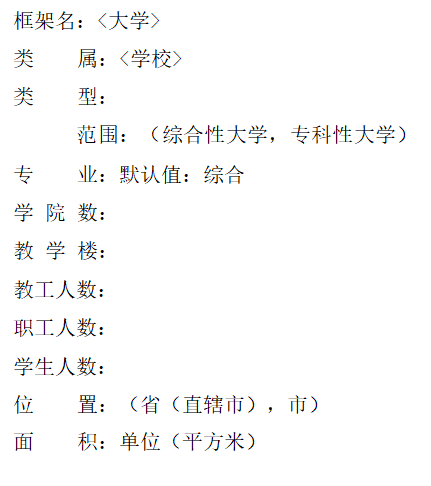
\includegraphics[scale = 0.5]{assets/ArtificialIntelligence_af860.png}
	\caption{类框架实例}
\end{figure}

\subsubsection{脚本表示法}
脚本方式是采用一个专用的框架,用来表示特定领域的知识。
脚本通过一些元语作为槽名来表代要表示的对象的基本行为。
有些像电影剧本。

包括:开场条件 , 场景 ,结果

脚本表使得知识有强烈的因果结构,系统对事件的处理必须是一个动作完成后才能完成另一个。整个过程的启动取决于开场条件,满足脚本的开场条件,脚本中的事件才有可能发生。而脚本的结果就是动作完成后的系统结果。

\subsection{过程表示法}
前面的几种知识表示方法均是知识和事实的一种静止的表示方法。我们称这类知识表示方式为陈述式表达。它所强调的是事物所涉及的对象是什么,是对事物有关知识的静态描述,是知识的一种显式、说明性知识表达形式。

说明性表示知识给出事物本身的属性及事物之间的相互关系。对问题的解答就隐含在这些知识之中。而过程性知识则给出解决一个问题的具体过程。

\textbf{说明性知识和过程性知识相比:}
\begin{itemize}
	\item 说明性知识比较简要、清晰、可靠、便于修改。但往往效率低。
	\item 过程性知识比较直截了当,效率高。但由于详细地给出了解决过程,使这种知识表示显得复杂、不直观、容易出错、不便于修改。
	\item 实际上,说明性表示和过程性表示实际上没有绝对的分界线。因此,任何说明性知识如果要被实际使用,必须有一个相应的过程去解释执行它。对于一个以使用说明性表示为主的系统来说,这种过程往往是隐含在系统之中,而不是面向用户。
\end{itemize}

\textbf{知识过程性的两个含义:}
\begin{itemize}
	\item 含义1:把解决一个问题的过程描述出来。可以称它为解题知识的过程表示。
	\item 含义2:把客观事物的发展过程用某种方式表示出来。
	\item 在某些情况下,这两种含义是很难决然分开的。如,任何一个解题系统的基本构成都是一个数据集,一组运算符和一个解释程序。过程性知识使用状态来表示,在状态空间运作。
\end{itemize}

\textbf{过程表示定义}:
\begin{itemize}
	\item 过程式表示就是将有关某一问题领域的知识连同如何使用这些知识的方法均隐式地表达为一个求解过程。
	\item 它所给出的是事物的一些客观规律,表达的是如何求解问题,知识的描述形式就是程序。所有信息均隐含在程序中——效率高、没有固定形式。
	\item 如何描述知识完全取决定于具体的问题。
\end{itemize}

\subsection{小结}
\begin{itemize}
	\item 谓词逻辑方法只适用于确定性、陈述性、静态性知识,而对动态的、变化性、模糊性知识则很难表示。
	\item 产生式规则方法推理方法太单一,如果前提条件太多,或规则条数太多,则推理的速度将慢得惊人。
	\item 语义网络方法表达的知识面比较窄。
	\item 框架方法表示的知识横向关系不太明确。(纵向从属继承关系很明确)
\end{itemize}

\section{不确定性推理}
\subsection{贝叶斯网络}
一系列变量的联合概率分布的图形表示。

一个表示变量之间的相互依赖关系的数据结构;图论与概率论的结合

贝叶斯网就是一个在弧的连接关系上加入连接强度的因果关系网络 。

\paragraph{贝叶斯网络由两个部分组成}
\begin{itemize}
	\item 贝叶斯网络结构图,这是一个有向无环图(DAG: Directed Acyclic Graph),其中图中的每个节点代表相应的变量。当有向弧由节点A指向节点B时,则称:A是B的父节点;B是A的子节点。
	\item 节点和节点之间的条件概率表(Conditional Probability Table, CPT),也就是一系列的概率值,表示了局部条件概率分布。P(node|parents) 。
\end{itemize}

\paragraph{目的} 由证据得出原因发生的概率。 即观察到P(Y),求$P(X|Y)$, 比如故障诊断

\paragraph{贝叶斯网络如何构造?}
\begin{itemize}
	\item 选择变量,生成节点
	\item 从左至右(从上到下),排列节点
	\item 填充网络连接弧,表示节点之间的关系
	\item 得到条件概率关系表
\end{itemize}

\paragraph{贝叶斯网络计算} 简单的联合概率可以直接从网络关系上得到

\begin{figure}[H]
	\centering
	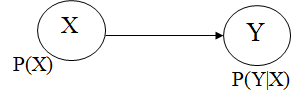
\includegraphics[scale = 0.3]{assets/ArtificialIntelligence/2018-01-08-23-03-30.png}
	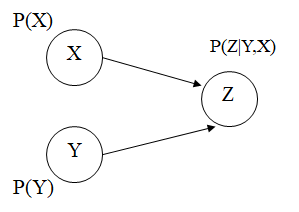
\includegraphics[scale = 0.3]{assets/ArtificialIntelligence/2018-01-08-23-04-22.png}
	\caption{$P(X,Y) = P(X)P(Y|X) ; P(X, Y, Z) = P(X)P(Y)P(Z|X, Y)$}
\end{figure}

\paragraph{条件独立}
对于X, Y, E: X与Y在给定E的条件下独立 , 有
\begin{itemize}
	\item $P(X|Y,E) = P(X|E)$
	\item $P(Y|X,E) = P(Y|E)$
\end{itemize}

\paragraph{D分离} 寻找条件独立的方法

\begin{figure}[H]
	\centering
	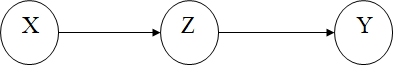
\includegraphics[scale = 0.3]{assets/ArtificialIntelligence/2018-01-08-23-14-07.png}
	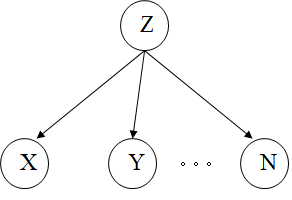
\includegraphics[scale = 0.3]{assets/ArtificialIntelligence/2018-01-08-23-14-35.png}
	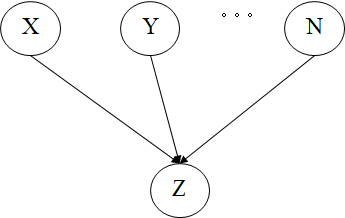
\includegraphics[scale = 0.3]{assets/ArtificialIntelligence/2018-01-08-23-14-43.png}
	\caption{D分离-串行;分叉连接 ; 汇集连接}
\end{figure}
\begin{itemize}
	\item 串行连接 : 事件X通过事件Z影响事件Y,反之事件Y也是通过事件Z影响事件X
	      \\ 但是,如果原因证据Z是给定的,X并不能给Y更多的东西,或者说,从X那里得到更多的信息。
	      \\此时称,如果Z是已知的,那么通道就被阻塞,X和Y就是独立的了。则称X和Y是被Z节点D分离的
	\item 分叉连接 : 父节点Z是已知的,没有更多的信息能够通过Z影响到所有子节点。同理,父节点Z是已知时,子节点X, …, N是相互独立的。称子节点X, …, N是被Z节点D分离的
	\item 汇集连接 : 如果不从父节点得到推断,子节点Z就一无所知,那么,父节点是相互独立的,它们之间没有相互影响。
	      \\如果,某事件影响了Z,那么,各个父节点就不是相互独立的了。该事件可以直接影响Z,也可以通过它的后代节点影响Z。这种现象称作条件依存。\\总之,如果子节点有了变化,或子节点的后代节点发生变化,信息是可以通过汇集连接传播的
\end{itemize}

\paragraph{贝叶斯网络的应用}
\begin{itemize}
	\item 因果推理X$\to$Y, 已知X,求P(Y)
	      \begin{itemize}
		      \item 按照给定证据的V和它的所有双亲的联合概率 , 重新表达给定证据的询问节点所求条件概率
		      \item 直到所有的概率值可从CPT表中得到, 推理完成
	      \end{itemize}
	\item 诊断推理X$\to$Y, 已知Y,求P(X)\\
	      使用贝叶斯定理可以把这种推理转换成因果推理
	\item 辩解推理X$\to$Y, Z$\to$Y,已知X,求P(Y)
\end{itemize}


\begin{figure}[H]
	\centering
	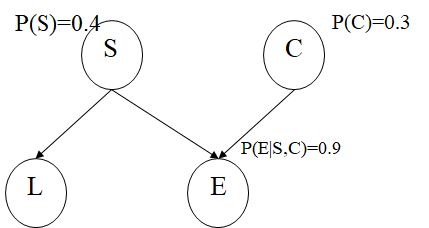
\includegraphics[scale = 0.3]{assets/ArtificialIntelligence/2018-01-08-23-05-56.png}
	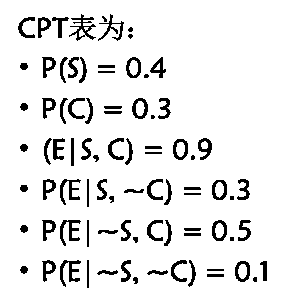
\includegraphics[scale = 0.3]{assets/ArtificialIntelligence/2018-01-08-23-07-31.png}
\end{figure}

\paragraph{例子}给定患者是一个吸烟者(S),计算他患肺气肿(E)的概率$P(E|S)$。S称作推理的证据,E叫询问结点。
\begin{itemize}
	\item 首先,E的另一个父结点(C),$P(E|S)=P(E,C|S)+P(E,\lnot C|S)$;
	\item 右边的第一项 ,
	      $P(E,C|S)=P(E,C,S)/P(S)=P(E|C,S)*P(C,S)/P(S)=P(E|C,S)*P(C)$
	\item 同理可得公式的右边的第二项为:$P(E,\lnot C|S) = P(E|\lnot C,S)*P(\lnot C)$。
	\item 由此可得:
	      $P(E|S)  =  P(E| C,S)*P(C)+P(E|\lnot C,S)*P(\lnot C)$
	\item 如果采用概述中的例题数据,有$P(\lnot C) = 1 - P(C)$,则有,
	      $P(E|S)=0.9*0.3+0.3*(1-0.3)=0.48$
\end{itemize}



\subsection{主观贝叶斯}
\paragraph{动机} 原有贝叶斯公式P(B|A),只考虑A出现对B的影响,没有考虑A不出现的影响。

\paragraph{规则的不确定性 - 充分性因子} : 表示A为真时,对B的影响(规则成立的充分性)
\[LS = \frac{P(A|B)}{P(A|\lnot B)} \]

\paragraph{规则的不确定性 - 必要性因子} : 表示A为假时,对B的影响(规则成立的必要性,确定性理论中没有考虑这点)
\[LS = \frac{P(\lnot A|B)}{\lnot P(A|\lnot B)} \]

\paragraph{几率函数}
\[O(X) = \frac{P(X)}{P(\lnot X)}\]

\paragraph{后验几率}
\[O(B|A) = \frac{P(B|A)}{P(\lnot B|A)}\]

那么LS可以改写成 : \textbf{后验几率与先验几率的比值}
\[LS = \frac{O(B|A)}{O(B)}\]

同理 ,LN 等价为:
\[LS = \frac{O(B|\lnot A)}{O(B)}\]

\begin{figure}[H]
	\centering
	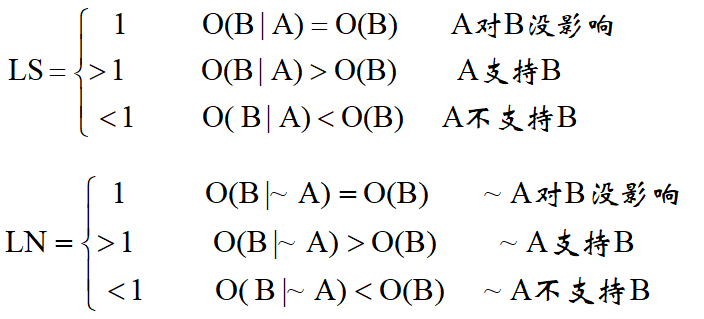
\includegraphics[scale = 0.3]{assets/ArtificialIntelligence/2018-01-08-23-45-51.png}
	\caption{LS , LN表示的规则的确定性程度}
\end{figure}

\paragraph{推理计算- A必然出现} 意味着$P(A) = 1$ , 接下来可以直接由(几率公式 而不是贝叶斯定理)公式计算出 $P(B|A)$

\paragraph{推理计算-A不确定} 向前看一步$A'$
\[P(B|A') = P(B|A)P(A|A') + P(B|\lnot A)P(\lnot A|A')\]
\begin{itemize}
	\item $P(A|A') = 1$ ,证据$A'$出现 , $A$必然出现
	      \begin{equation}
		      \begin{array}{ll}
			      P(B|A) & = \displaystyle\frac{P(B|A)}{P(B|A) + P(\lnot B|A)}                                         \\
			             & = \displaystyle\frac{P(B|A)P(A)}{P(B|A)P(A) + P(\lnot B|A)P(A)}                             \\
			             & = \displaystyle\frac{P(AB)}{P(AB) + P(A\lnot B)}                                            \\
			             & = \displaystyle\frac{P(AB)}{P(AB) + P(A|\lnot B)P(\lnot B)}                                      \\
			             & = \displaystyle\frac{P(AB)}{P(AB) + P(A|\lnot B)-P(A|\lnot B)P(B)}                               \\
			             & = \displaystyle\frac{\frac{P(A|B)}{P(A|\lnot B)}P(B)}{(\frac{P(A|B)}{P(A|\lnot B)} - 1)P(B) + 1} \\
			             & = \displaystyle\frac{LS \times P(B)}{(LS - 1)\times P(B) + 1}
		      \end{array}
	      \end{equation}
	\item  $P(A|A') = 0$ ,证据$A'$出现 , $A$必然 \textbf{不} 出现 ,同理
	      \[P(B|A') = P(B|\lnot A) = \frac{LN \times P(B)}{(LS - 1)\times P(B) + 1}\]
	\item $P(A|A') = P(A)$ 时 , $A'$对$A$ 没有影响 \\
	      \[P(B|A') = P(B)\]
\end{itemize}

思路:先定好应该怎么办,再凑公式。主要是避开P(A| B)的计算。

由上面三点 , 拟合$P(A|A')$和$P(B|A')$的关系:
\begin{figure}[H]
	\centering
	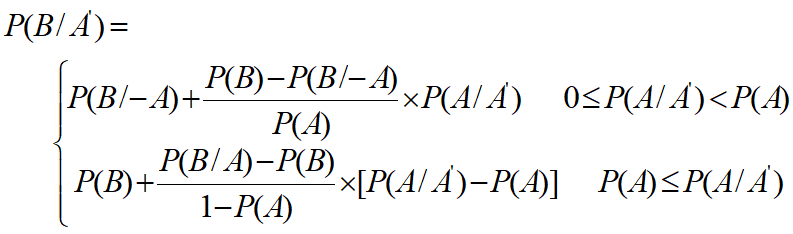
\includegraphics[scale = 0.3]{assets/ArtificialIntelligence/2018-01-09-00-11-12.png}
	\caption{插值计算公式}
\end{figure}

\begin{figure}[H]
	\centering
	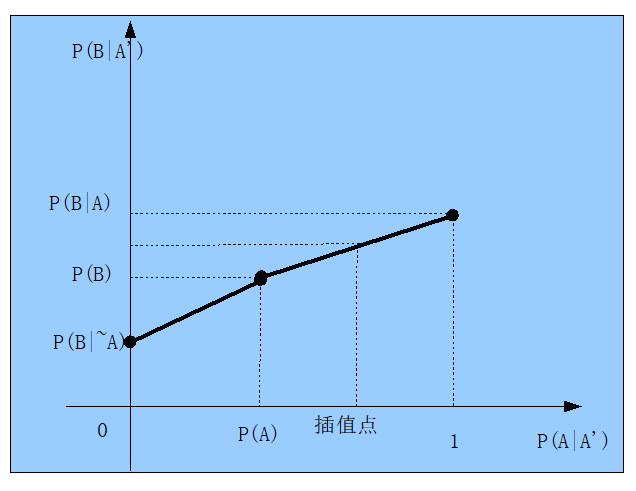
\includegraphics[scale = 0.3]{assets/ArtificialIntelligence/2018-01-09-00-11-35.png}
	\caption{线性插值图}
\end{figure}

\paragraph{证据合成} 当有两个证据$A_1 , A_2$和观测证据$A'$ ,($A' \to A_1 \land A_2$)

\begin{figure}[H]
	\centering
	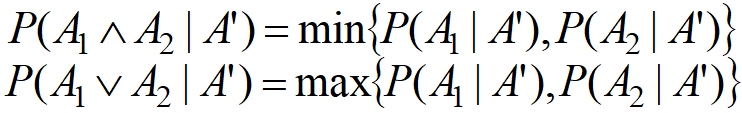
\includegraphics[scale = 0.3]{assets/ArtificialIntelligence/2018-01-09-00-16-44.png}
\end{figure}


\paragraph{证据组合} 互相独立证据导出同一假设($A_1 \to B , A_2 \to B$)
\begin{figure}[H]
	\centering
	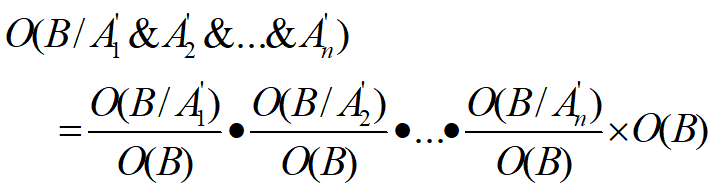
\includegraphics[scale = 0.3]{assets/ArtificialIntelligence/2018-01-09-00-17-49.png}
\end{figure}

\paragraph{习题}
\begin{figure}[H]
	\centering
	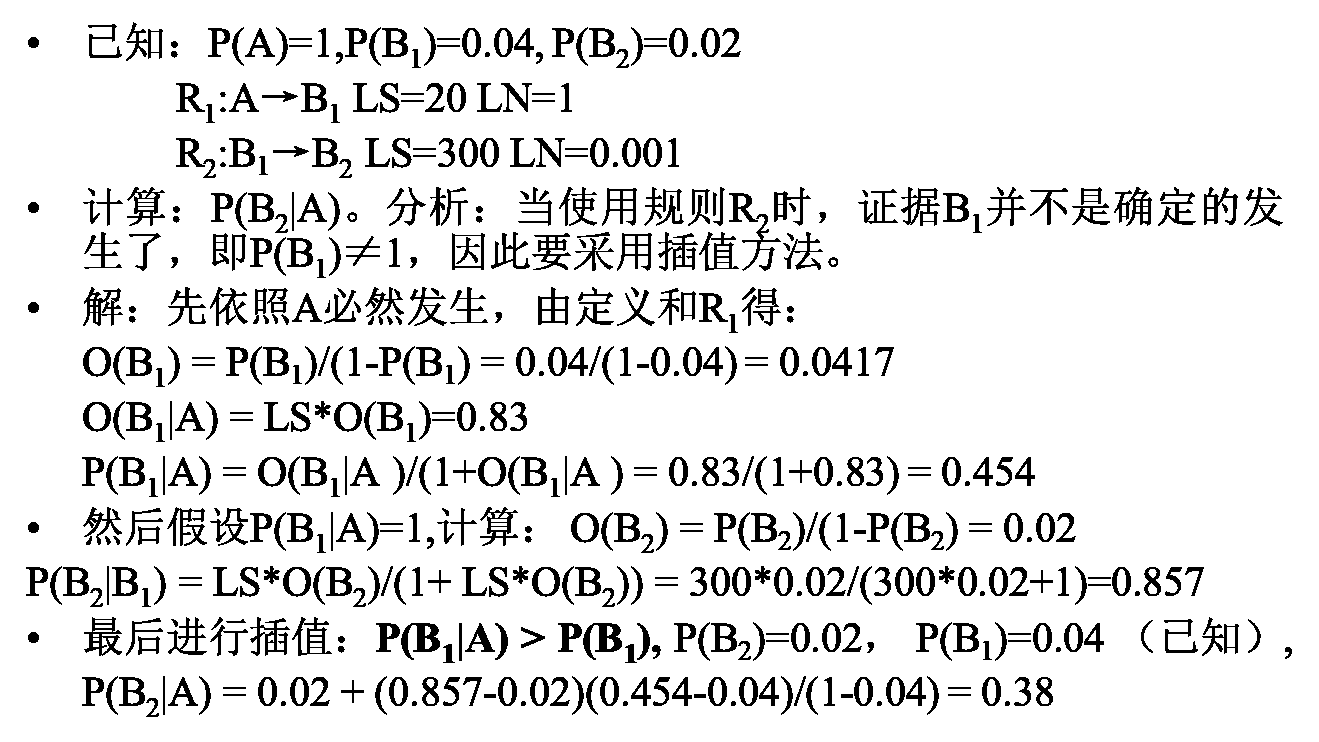
\includegraphics[scale = 0.3]{assets/ArtificialIntelligence/2018-01-09-00-20-13.png}
	\caption{主观贝叶斯 - 例题1}
\end{figure}

\begin{figure}[H]
	\centering
	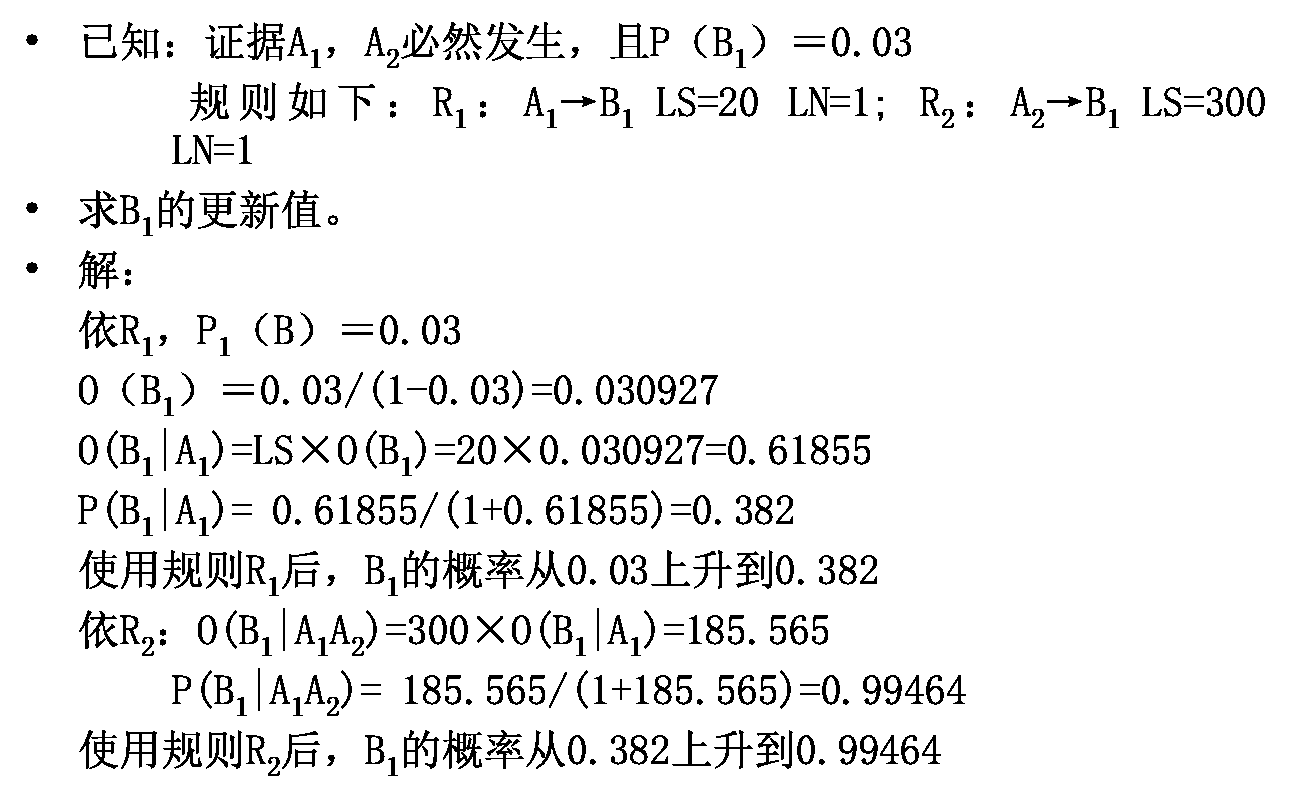
\includegraphics[scale = 0.3]{assets/ArtificialIntelligence/2018-01-09-00-20-53.png}
	\caption{主观贝叶斯 - 例题2}
\end{figure}

\subsection{确定性方法}

\paragraph{规则的不确定性度量}
\begin{figure}[H]
	\centering
	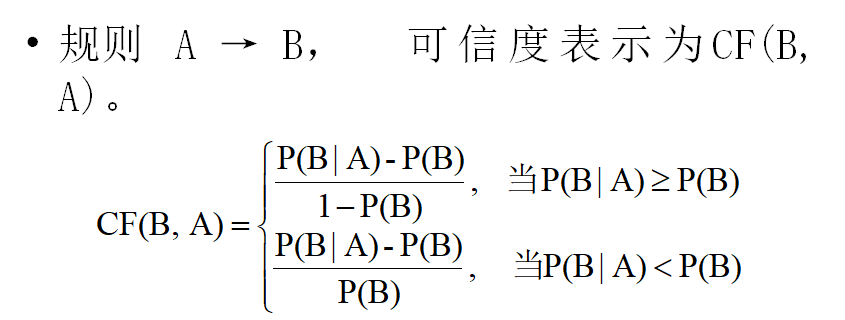
\includegraphics[scale = 0.3]{assets/ArtificialIntelligence/2018-01-09-00-23-04.png}
\end{figure}
\paragraph{CF(B, A)表示的意义}
\begin{itemize}
	\item 证据为真时相对于$P(\lnot B) = 1 - P(B)$来说,A对B为真的支持程度。即A发生更支持B发生。
	      此时 CF(B, A)≥ 0。
	\item 或,相对于P(B)来说,A对B为真的不支持程度。即A发生不支持B发生。
	      此时 CF(B, A)< 0。
\end{itemize}

\paragraph{CF(B, A)的特殊值:}
\begin{itemize}
	\item CF(B, A) = 1,	前提真,结论必真
	\item CF(B, A) = -1,前提真,结论必假
	\item CF(B, A) = 0 , 前提真假与结论无关
	\item CF( A) > 0, 表示A以CF( A)程度为真
	\item CF( A) < 0, 表示A以CF( A)程度为假
\end{itemize}

\begin{figure}[H]
	\centering
	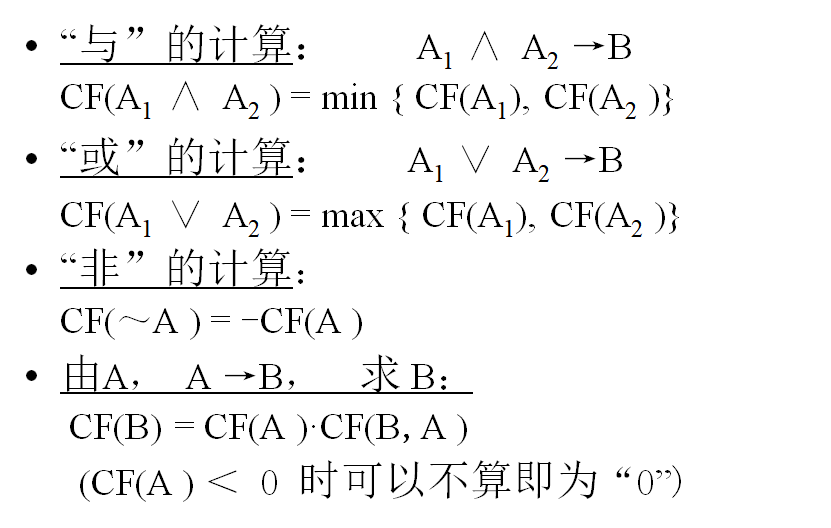
\includegraphics[scale = 0.5]{assets/ArtificialIntelligence/2018-01-09-00-27-15.png}
	\caption{推理计算}
\end{figure}

\begin{figure}[H]
	\centering
	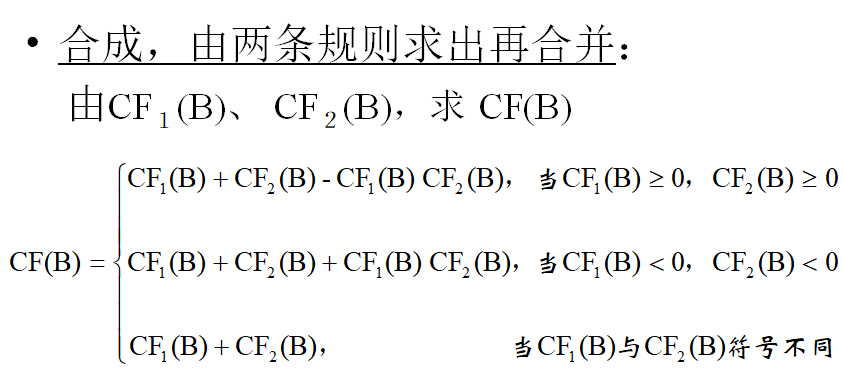
\includegraphics[scale = 0.5]{assets/ArtificialIntelligence/2018-01-09-00-27-49.png}
\end{figure}

\begin{figure}[H]
	\centering
	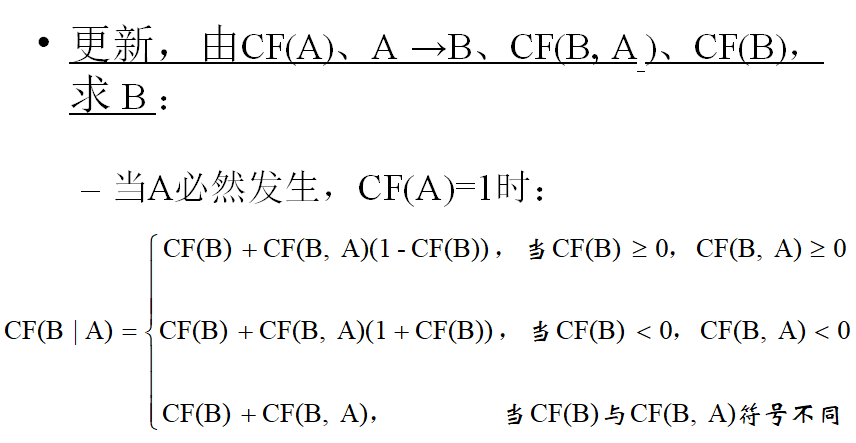
\includegraphics[scale = 0.5]{assets/ArtificialIntelligence/2018-01-09-00-28-10.png}
\end{figure}

\begin{figure}[H]
	\centering
	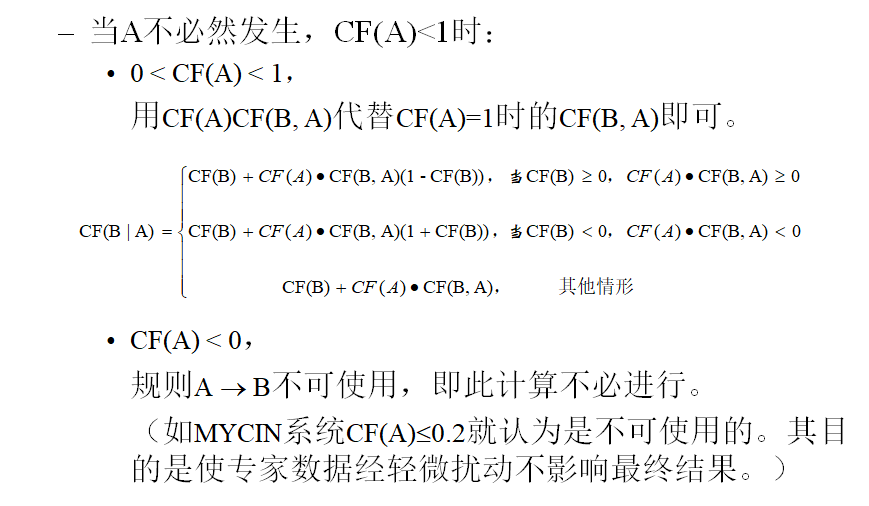
\includegraphics[scale = 0.5]{assets/ArtificialIntelligence/2018-01-09-00-28-36.png}
\end{figure}

\begin{figure}[H]
	\centering
	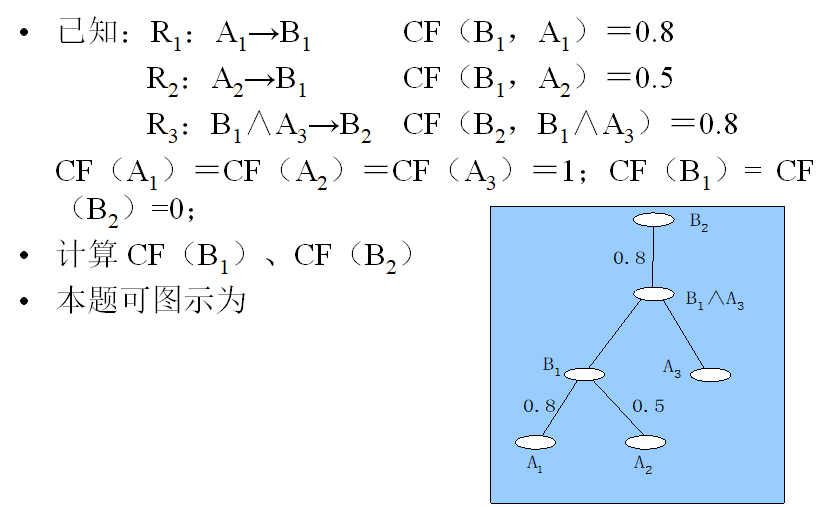
\includegraphics[scale = 0.5]{assets/ArtificialIntelligence/2018-01-09-00-29-14.png}
	\caption{例题}
\end{figure}

\begin{figure}[H]
	\centering
	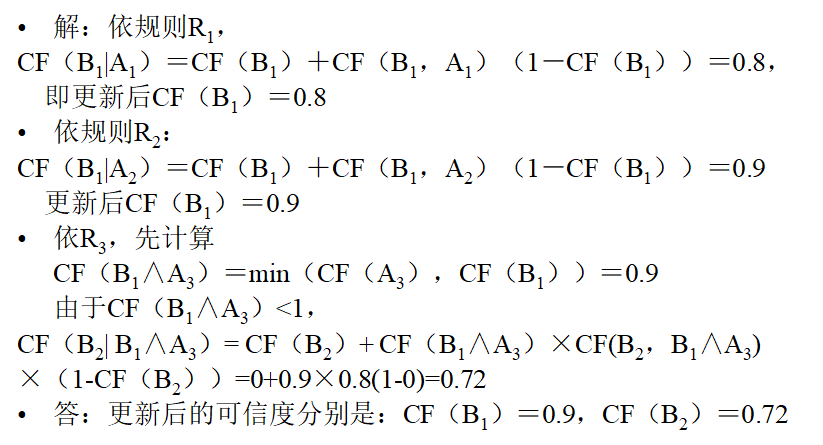
\includegraphics[scale = 0.5]{assets/ArtificialIntelligence/2018-01-09-00-29-43.png}
	\caption{例题解答}
\end{figure}


\subsection{证据理论}

\paragraph{基本概率分配函数}: m(A)表示了证据对U的子集A成立的一种信任度
\[m(\phi) = 0 , \sum_{A \sqsubseteq U}m(A) = 1\]

\paragraph{信任函数} Bel类似于概率密度函数,表示A中所有子集的基本概率分配数值的和,用来表示对A的总信任度。
\[Bel(A) = \sum_{B \subseteq A} m(B)\]

\paragraph{似然函数}
\[Pl(A) = 1 - Bel(\lnot A) = \sum_{B \cup A \neq \phi} m(B)\]

Bel(A)和Pl(A)是A的下限不确定性值和上限不确定性值。

\paragraph{综合Bel(A) , Pl(A) 来衡量A的不确定性}:
\[f_1(A) = Bel(A) + \frac{|A|}{|U|}(Pl(A) - Bel(A))\]

\paragraph{推理计算}设子集合A、B,其中A = {a1, a2, …, ak},
B = {b1, b2, …, bk},
用相应的向量(c1, c2, …, ck)描述规则A$\to$B的不确定性度量,
其中:ci≥0, 1≤i≤k, 且∑cj≤1, 1≤j≤k

已知事件A,由f1(A)求bk, bk = f1(A)ck

\begin{figure}[H]
	\centering
	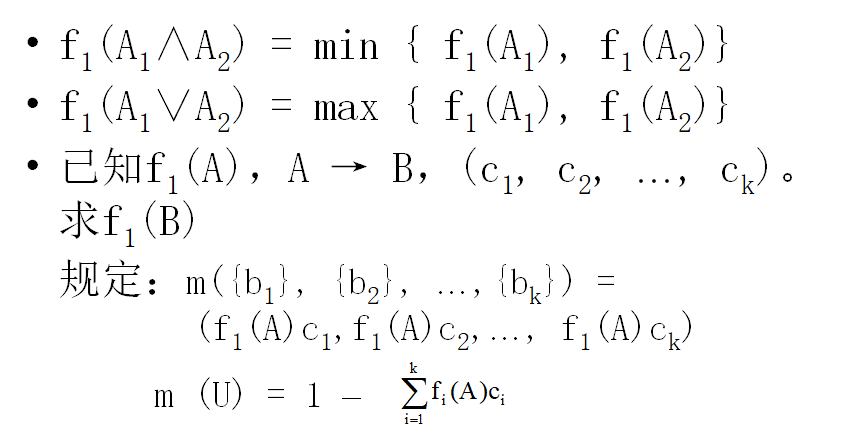
\includegraphics[scale = 0.5]{assets/ArtificialIntelligence/2018-01-09-00-44-55.png}
	\caption{推理计算}
\end{figure}

\begin{figure}[H]
	\centering
	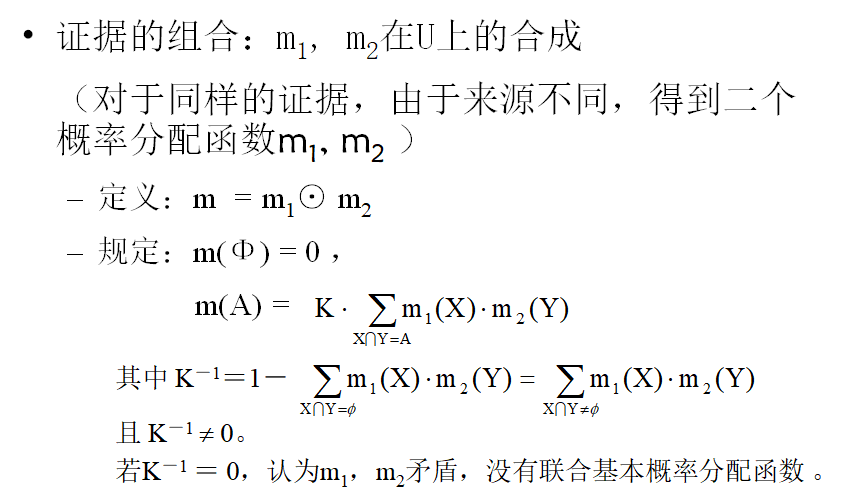
\includegraphics[scale = 0.5]{assets/ArtificialIntelligence/2018-01-09-00-46-51.png}
	\caption{证据组合}
\end{figure}

\begin{figure}[H]
	\centering
	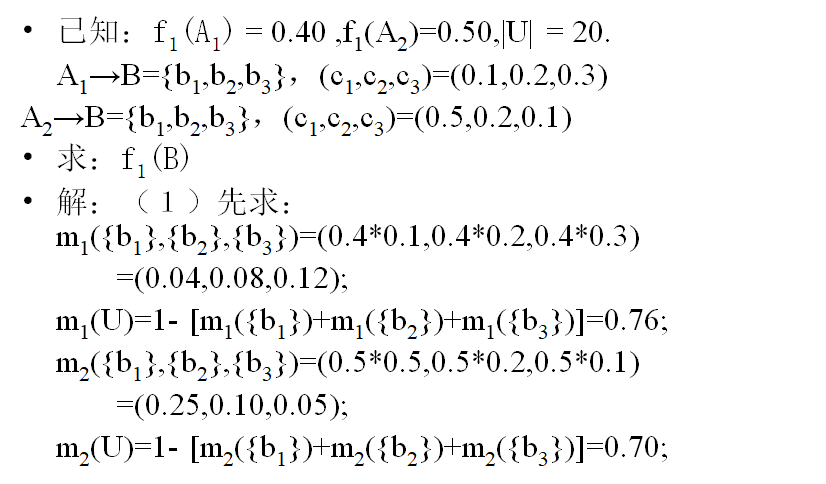
\includegraphics[scale = 0.5]{assets/ArtificialIntelligence/2018-01-09-00-47-51.png}
\end{figure}
\begin{figure}[H]
	\centering
	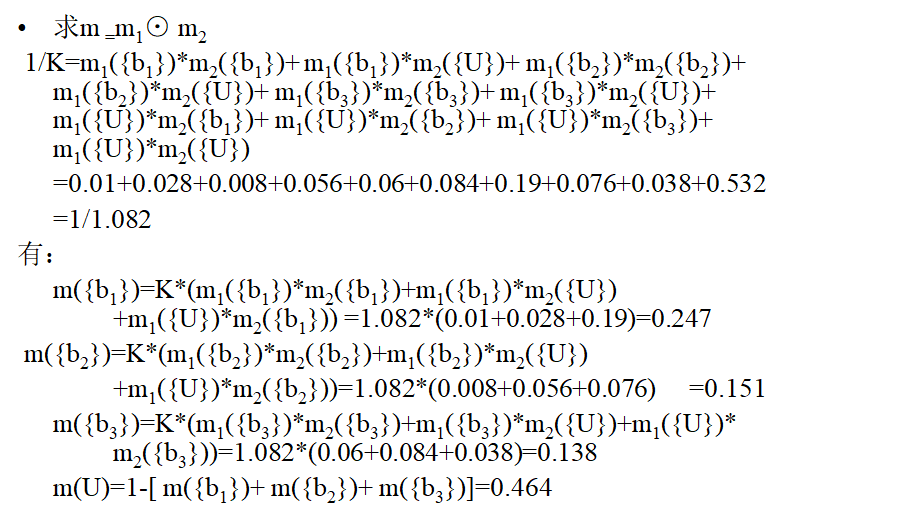
\includegraphics[scale = 0.5]{assets/ArtificialIntelligence/2018-01-09-00-48-11.png}
\end{figure}
\begin{figure}[H]
	\centering
	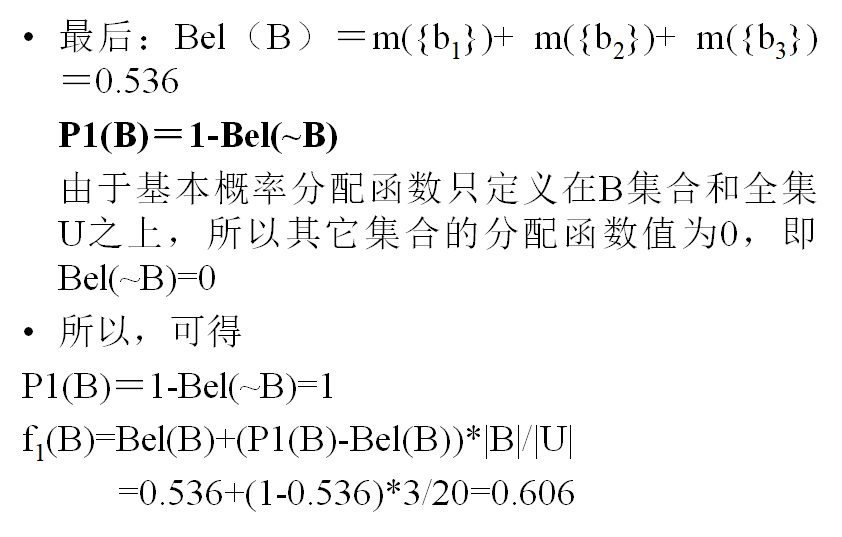
\includegraphics[scale = 0.5]{assets/ArtificialIntelligence/2018-01-09-00-48-30.png}
\end{figure}


\section{机器学习}
\paragraph{什么是机器学习?}
学习是一种具有多侧面的现象。学习的过程有:获取新的陈述性知识、通过教育或实践发展机械技能和认知能力、将新知识组织成为通用化和有效的表达形式、借助观察和实验发现新的事实和新的理论。

Simon(1983):学习就是系统中的变化,这种变化使系统比以前更有效地去做同样的工作。

Minsky (1985):学习是在我们头脑中(心里内部)进行有用的变化。

\paragraph{机器学习分类}(按学习策略分类)
\begin{itemize}
	\item 机械式学习,直接输入新知识(记忆学习)
	      学习者不需要进行任何推理或知识转换,将知识直接装进机器中。
	\item 根据示教学习(such as Classification)
	      从老师或其它有结构的事物获取知识。要求学习者将输入语言的知识转换成它本身的内部表示形式。并把新的信息和它原有的知识有机地结合为一体。
	\item 通过类推学习(演绎学习)
	      学习者找出现有知识中所要产生的新概念或技能十分类似的部分。将它们转换或扩大成适合新情况的形式,从而取得新的事实或技能。
	\item 从例子中学习(归纳学习)
	      给学习者提供某一概念的一组正例和反例,学习者归纳出一个总的概念描述,使它适合于所有的正例且排除所有的反例。(目前研究较多的一种方法)Classification and Prediction
	\item 类比学习
	      演绎学习与归纳学习的组合。匹配不同论域的描述、确定公共的结构。以此作为类比映射的基础。寻找公共子结构是归纳推理,而实现类比映射是演绎推理。
\end{itemize}

\begin{figure}[H]
	\centering
	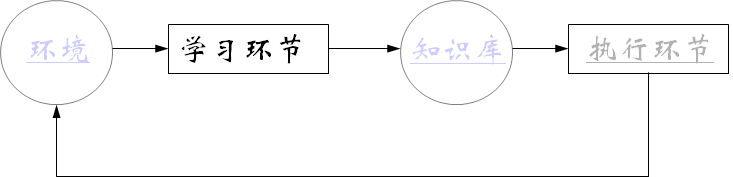
\includegraphics[scale = 0.3]{assets/ArtificialIntelligence/2018-01-09-00-54-20.png}
	\caption{机器学习模型}
\end{figure}

学习是建立理论、形成假设和进行归纳推理的过程。

\subsection{实例学习}
\paragraph{变形空间法}
\begin{itemize}
	\item 变形空间方法以整个规则空间为初始的假设规则集合H。依据示教例子中的信息,对集合H进行一般化或特殊化处理。逐步缩小集合H,最后使H收敛为只含有要求的规则
	\item 由于被搜索的空间H逐步缩小,故称为变形空间。
\end{itemize}

\paragraph{具体方法}消除候选元素法
\begin{itemize}
	\item 正例去掉G中不符合的概念,然后修改S ,归纳出最特殊的结果,尽量少改S。
	\item    反例去掉S中符合的概念,然后修改G,做特殊化得到最一般的结果,尽量少改G.
\end{itemize}

\subsection{决策树学习}
\paragraph{决策树(Decision Tree)}
一种描述概念空间的有效的归纳推理办法。基于决策树的学习方法可以进行不相关的多概念学习,具有简单快捷的优势,已经在各个领域取得广泛应用。

通用的决策树分裂目标是整棵树的熵总量最小,每一步分裂时,选择使熵减小最大的准则,这种方案使最具有分类潜力的准则最先被提取出来

\paragraph{信息熵}
\[\mathrm{H} (X)=\sum _{{i}}{{\mathrm  {P}}(x_{i})\,{\mathrm  {I}}(x_{i})}=-\sum _{{i}}{{\mathrm  {P}}(x_{i})\log _{b}{\mathrm  {P}}(x_{i})}\]

\paragraph{条件熵}
\[{\displaystyle \mathrm {H} (X|Y)=-\sum _{i,j}p(x_{i},y_{j})\log {\frac {p(x_{i},y_{j})}{p(y_{j})}}}\]

\paragraph{ID3算法}ID3将信息熵下降速度作为属性选择标准

\begin{itemize}
	\item 使用所有没有使用的属性并计算与之相关的样本熵值
	\item 选取其中熵值(条件熵最小 , 代表选择该属性后,熵下降自最多)最小的属性
	\item 生成包含该属性的节点
\end{itemize}

\paragraph{决策树的优点}
\begin{itemize}
	\item 	可以生成可以理解的规则;
	\item 计算量相对来说不是很大;
	\item 可以处理连续和离散字段;
	\item 决策树可以清晰的显示哪些字段比较重要
\end{itemize}

\paragraph{决策树的不足}
\begin{itemize}
	\item 对连续性的字段比较难预测
	\item 当类别太多时,错误可能会增加的比较快
	\item 一般的算法分类的时候,只是根据一个属性来分类。
	\item 不是全局最优。
\end{itemize}

\subsection{神经网络}
\paragraph{什么叫人工神经网络}采用物理可实现的系统来模仿人脑神经细胞的结构和功能的系统。

\paragraph{人工智能于神经网络}:
\subparagraph{共同之处}:研究怎样使用计算机来模仿人脑工作过程。学习——实践——再学习——再实践 。
\subparagraph{不同之处}:
人工智能研究人脑的推理、学习、思考、规划等思维活动,解决需人类专家才能处理的复杂问题。
神经网络企图阐明人脑结构及其功能,以及一些相关学习、联想记忆的基本规则(联想、概括、并行搜索、学习和灵活性)

\paragraph{网络模型}
\begin{itemize}
	\item {前馈神经网络} 每层只与前层相联接

	\item{有反馈的前向网络} 输出层上存在一个反馈回路,将信号反馈到输入层。而网络本身还是前馈型的

	\item{前馈内层互联网络} 外部看还是一个前向网络,内部有很多自组织网络在层内互联着。

	\item{反馈型全互联网络}所有计算单元之间都有联接。如:Hopfield网络

\end{itemize}

\paragraph{网络分类}前馈型  ; 反馈型 ; 自组织竞争型 ; 随机网络 ; 其他

\paragraph{神经网络的基本属性}
\begin{itemize}
	\item 非线性性:非线性关系是自然界的普遍特性。大脑的智慧就是一种非线性现象。人工神经元处于激活或抑制两种不同的状态。这种行为在数学上表现为一种非线性
	\item 非局域性 : 一个神经网络通常由多个神经元广泛联接而成。一个系统的整体行为不仅取决于单个神经元的特征,而且可能主要由单元之间的相互作用、相互联接所决定。通过单元之间的大量联接模拟大脑的非局域性。联想记忆是非局域性的典型例子。
	\item 非定常性 : 人工神经网络具有自适应、自组织、自学习能力。神经网络不但处理的信息有各种各样,而且在处理信息的同时,非线性动力系统本身也在不断变化。经常采用迭代过程描写动力系统的演化过程。
	\item 非凸性 : 一个系统的演化方向,在一定条件下,将取决于某个特定的状态函数,如能量函数,它的极值相应于系统比较稳定的状态。非凸性是指这种函数有多个极值,故系统具有多个较稳定的平衡态,这将导致系统演化的多样性。
\end{itemize}

\paragraph{优点} : 并行性;分布存储;容错性;学习能力

\paragraph{缺点} : 不适合高精度计算;学习问题没有根本解决,慢;目前没有完整的设计方法,经验参数太多。

\subsubsection{BP网络}
\paragraph{BP算法基本原理}
利用输出后的误差来估计输出层的直接前导层的误差,再用这个误差估计更前一层的误差,如此一层一层的反传下去,就获得了所有其他各层的误差估计。

\paragraph{BP网络的特点}
\begin{itemize}
	\item 非线性映射能力:
	      能学习和存贮大量输入-输出模式映射关系,而无需事先了解描述这种映射关系的数学方程。只要能提供足够多的样本模式对供网络进行学习训练,它便能完成由n维输入空间到m维输出空间的非线性映射。
	\item 泛化能力:
	      当向网络输入训练时未曾见过的非样本数据时,网络也能完成由输入空间向输出空间的正确映射。这种能力称为泛化能力
	\item 容错能力:
	      输入样本中带有较大的误差甚至个别错误对网络的输入输出规律影响很小。
\end{itemize}

\subsubsection{自组织竞争人工神经网络}
在实际的神经网络中,存在一种侧抑制的现象。即一个细胞兴奋后,通过它的分支会对周围其他神经细胞产生抑制。这种侧抑制在脊髓和海马中存在,在人眼的视网膜中也存在。

这种抑制使神经细胞之间出现竞争,一个兴奋最强的神经细胞对周围神经细胞的抑制也强。虽然一开始各个神经细胞都处于兴奋状态,但最后是那个输出最大的神经细胞“赢”,而其周围的神经细胞“输”了。

自组织神经网络特别适合于解决模式分类和识别方面的应用问题。

自组织神经网络属于前向神经网络类型,采用无导师学习算法,

自组织特征映射神经网络不仅能够像自组织竞争神经网络一样学习输入的分布情况,而且可以学习神经网络的拓扑结构

\paragraph{自组织竞争神经网络类型}
\begin{itemize}
	\item 自适应共振理论(Adaptive Resonance Theory,ART)网络
	\item 自组织特征映射(self-Organizing Map,SOM)网络
	\item 对传(Counter Propagation,CP)网络
	\item 协同神经网络(Synergetic Neural Network.SNN)
\end{itemize}

\paragraph{自组织特征映射神经网络结构 SOM}
由芬兰学者Teuvo Kohonen于1981年提出,基本上为输入层和映射层的双层结构,映射层的神经元互相连接,每个输出神经元连接至所有输入神经元
\begin{figure}[H]
	\centering
	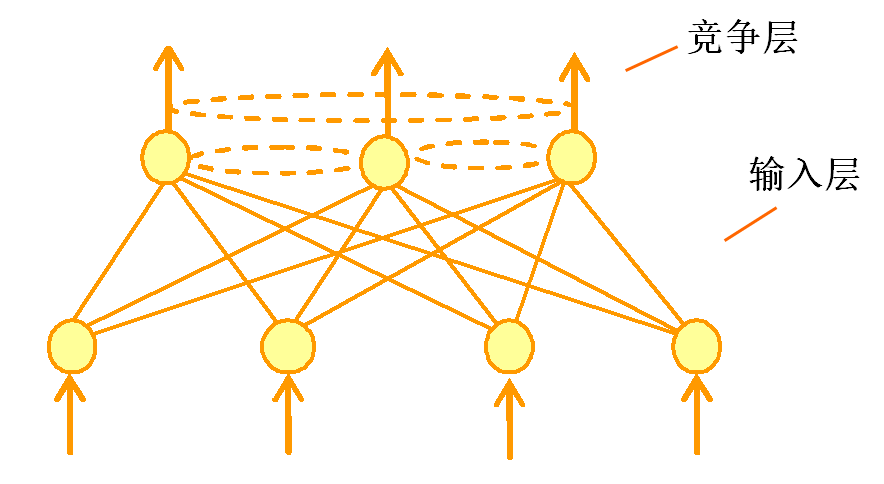
\includegraphics[scale = 0.3]{assets/ArtificialIntelligence/2018-01-09-13-59-31.png}
	\caption{SOM神经网络结构}
\end{figure}

\paragraph{网络形成过程}
开始是无序的,当输入样本出现后各个细胞反映不同,强者依照“胜者为王”的原则,加强自己的同时对周围细胞进行压抑。使其对该种样本更加敏感,也同时对其他种类的样本更加不敏感。此过程的反复过程中,各种不同输入样本将会分别映射到不同的细胞上

\paragraph{自组织特征映射学习算法原理}
Kohonen自组织特征映射算法,能够自动找出输入数据之间的类似度,将相似的输入在网络上就近配置。因此是一种可以构成对输入数据有选择地给予响应的网络

\paragraph{自组织特征映射学习算法步骤}
\begin{itemize}
	\item 网络初始化\\
	      用随机数设定输入层和映射层之间权值的初始值
	\item 输入向量\\
	      把输入向量输入给输入层
	\item 计算映射层的权值向量和输入向量的距离\\
	      映射层的神经元和输入向量的距离,按下式给出
	      \[d_j = \sqrt{\displaystyle{\sum_{i  =1}^n} (x_i - w_{ij})^2}\]
	\item 选择与权值向量的距离最小的神经元\\
	      计算并选择使输入向量和权值向量的距离最小的神经元,把其称为胜出神经元并记为 j ,并给出其邻接神经元集合。
	\item 调整权值 \\
	      胜出神经元和位于其邻接神经元的权值,按下式更新:
	      \[\Delta w_{ij}= \eta h(j , j^*)(x_i - w_{ij})\]
	      \[w_{ij}(t + 1) = w_{ij}(t) + \Delta w_{ij}\]

	\item 是否达到预先设定的要求如达到要求则算法结束,否则返回第二步,进入下一轮学习
\end{itemize}

\paragraph{网络学习的结果是}比较相近的输入样本在输出平面上映射的位置也比较接近。具有自然聚类的效果。

\paragraph{邻域函数}
\[h(j , j^*) = exp(-\frac{|j-j^*|^2}{\sigma^2})\]

\section{高级搜索}
很多问题属于优化问题,或者可以转化为优化问题

\paragraph{优化问题的描述}
设x是决策变量,D是x的定义域,f(x)是指标函数,g(x)是约束条件集合。则优化问题可以表示为,求解满足g(x)的f(x)最小值问题。
\[\min_{	x \in D} (f(x)|g(x))\]
如果在定义域D上,满足条件g(x)的解是有限的,则优化问题称为组合优化问题

\subsection{局部搜索}
\paragraph{基本思想}在搜索过程中,始终向着离目标最接近的方向搜索。
目标可以是最大值,也可以是最小值。

\paragraph{具体过程} 搜索过程 , 不断在最优点邻域内选择新的最优点 ,直到最优点不再变化

\paragraph{存在的问题}
\begin{itemize}
	\item 局部最优问题
	      \paragraph{解决办法} 每次并不一定选择邻域内最优的点,而是依据一定的概率,从邻域内选择一个点,指标函数优的点,被选中的概率比较大,而指标函数差的点,被选中的概率比较小。
	\item 步长问题
	      \paragraph{解决办法}变步长

	\item 起始点问题
	      \paragraph{解决办法}随机的生成一些初始点,从每个初始点出发进行搜索,找到各自的最优解。再从这些最优解中选择一个最好的结果作为最终的结果。
\end{itemize}

\subsection{模拟退火}
将局部搜索算法中存在的问题的 	第一、第二种方法的结合就产生了模拟退火方法。

\paragraph{溶解过程}随着温度的不断上升,粒子逐渐脱离开其平衡位置,变得越来越自由,直到达到固体的溶解温度,粒子排列从原来的有序状态变为完全的无序状态。
\paragraph{退火过程}随着温度的下降,粒子的热运动逐渐减弱,粒子逐渐停留在不同的状态,其排列也从无序向有序方向发展,直至到温度很低时,粒子重新以一定的结构排列

粒子不同的排列结构,对应着不同的能量水平。如果退火过程是缓慢进行的,也就是说,温度的下降如果非常缓慢的话,使得在每个温度下,粒子的排列都达到一种平衡态,则当温度趋于0(绝对温度)时,系统的能量将趋于最小值

如果以粒子的排列或者相应的能量来表达固体所处的状态,在温度T下,固体所处的状态具有一定的随机性。一方面,物理系统倾向于能量较低的状态,另一方面,热运动又妨碍了系统准确落入低能状态。

\begin{figure}[H]
	\centering
	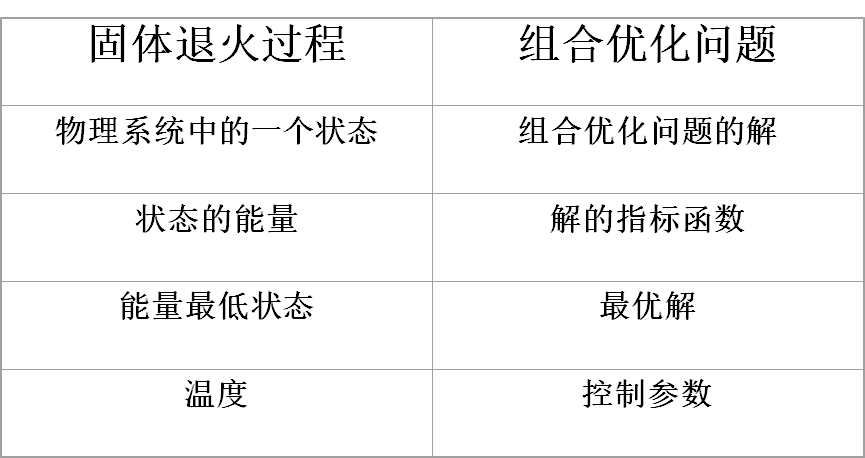
\includegraphics[scale = 0.3]{assets/ArtificialIntelligence/2018-01-09-14-21-51.png}
	\caption{组合优化问题与退火过程的类比}
\end{figure}

\paragraph{每一温度下的停止准则}
\begin{itemize}
	\item 固定长度方法
	\item 基于接受率的停止准则
	\item 零度法
	\item 循环总控制法
	\item 无变化控制法
	\item 接受概率控制法
	\item 领域平均概率控制法
\end{itemize}
\subsection{遗传算法}
\begin{figure}[H]
	\centering
	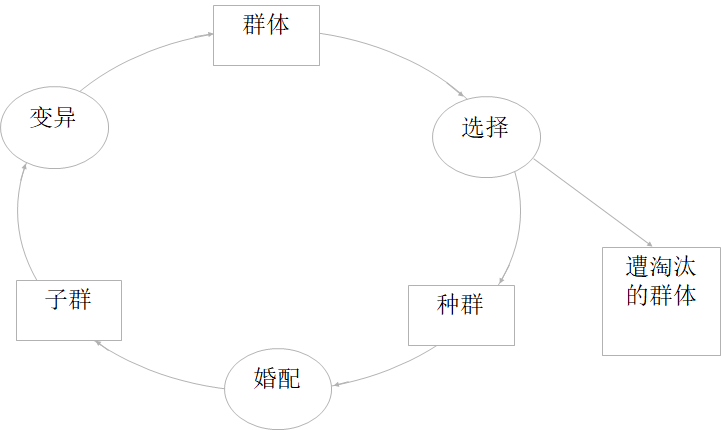
\includegraphics[scale = 0.5]{assets/ArtificialIntelligence/2018-01-09-14-25-06.png}
	\caption{生物进化与遗传算法 }
\end{figure}

\begin{figure}[H]
	\centering
	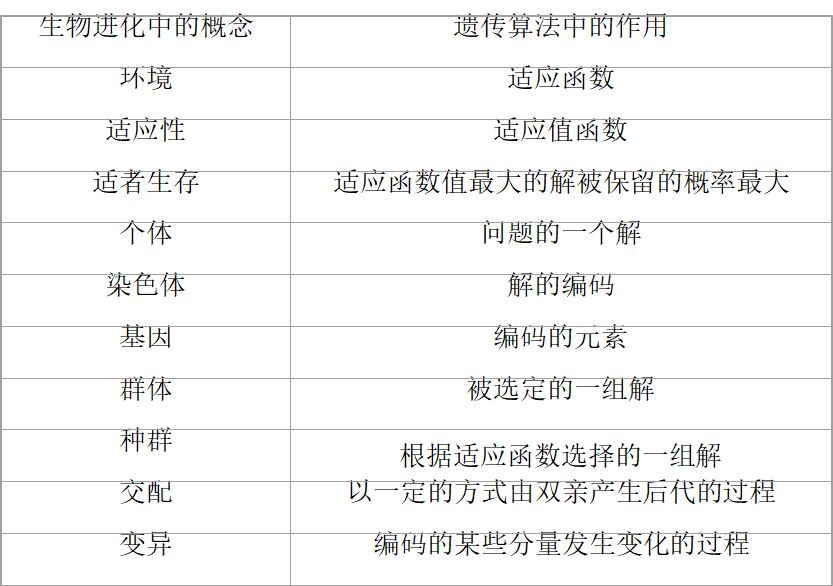
\includegraphics[scale = 0.5]{assets/ArtificialIntelligence/2018-01-09-14-25-26.png}
	\caption{生物进化与遗传算法之间的对应关系 }
\end{figure}

\paragraph{遗传算法的3个主要操作} 选择;交配;变异

\begin{itemize}
	\item 选择
	      \paragraph{转轮法} : 以适应值作为计算量, 得出每个染色体被选择的概率
	      \[p(x_i) = \frac{F(x_i)}{\displaystyle{\sum_{j = 1}^B F(x_j)} }\]
	      \paragraph{确定性选择} : 以被选择的概率计算出每个染色体被选择次数的期望 , 选择前N个期望最大的染色体
\end{itemize}

遗传算法是一个随机搜索算法,适用于数值求解具有多参数、多变量、多目标等复杂的最优化问题。

\paragraph{二进制编码的交配规则 }
\begin{itemize}
	\item 双亲双子法
	      \begin{figure}[H]
		      \centering
		      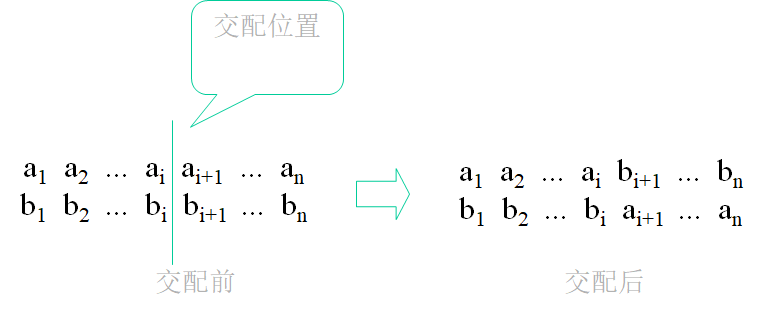
\includegraphics[scale = 0.5]{assets/ArtificialIntelligence/2018-01-09-14-33-35.png}
	      \end{figure}
	\item 变化交配法 :
	      变化交配法就是在随机产生交配位时,排除掉染色体位相同的交配位。
	\item 多交配位法
	      \begin{figure}[H]
		      \centering
		      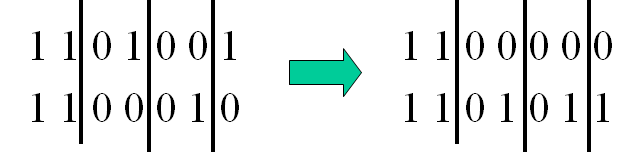
\includegraphics[scale = 0.3]{assets/ArtificialIntelligence/2018-01-09-14-36-19.png}
	      \end{figure}

\end{itemize}

\paragraph{整数编码的交配规则 } 以旅行商为例
\begin{itemize}
	\item 随机选取交配位,子代1: 交配位之前的基因选自父代1交配位之前的基因,交配位之后的基因,从父代2中按顺序选取那些在子代1中还没有出现过的基因。
	      \begin{figure}[H]
		      \centering
		      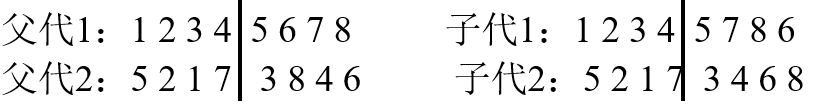
\includegraphics[scale = 0.3]{assets/ArtificialIntelligence/2018-01-09-14-40-57.png}
		      \caption{子代1前4位一样 , 后4位的顺序由父代2的顺序决定}
	      \end{figure}
	\item 基于次序的交配法
	      \begin{figure}[H]
		      \centering
		      \includegraphics[scale = 0.5]{assets/ArtificialIntelligence/2018-01-09-14-43-07.png}
		      \caption{基于次序的交配法}
	      \end{figure}

	\item 基于位置的交配方法
	      \begin{figure}[H]
		      \centering
		      \includegraphics[scale = 0.3]{assets/ArtificialIntelligence/2018-01-09-14-43-36.png}
		      \caption{基于位置的交配方法}
	      \end{figure}
	\item 基于部分映射的交配法
	      \begin{figure}[H]
		      \centering
		      \includegraphics[scale = 0.3]{assets/ArtificialIntelligence/2018-01-09-14-44-05.png}
		      \caption{基于部分映射的交配法 }
	      \end{figure}
\end{itemize}

\paragraph{二进制编码中的变异}当问题以二进制编码形式表示时,随机的产生一个变异位,被选中的基因由“0”变为“1”,或者由“1”变为“0”

\paragraph{整数编码中的变异}
\begin{itemize}
	\item 于位置的变异:
	      随机的产生两个变异位,然后将第二个变异位上的基因移动到第一变异位之前
	\item 基于次序的变异 : 随机的产生两个变异位,然后交换这两个变异位上的基因。
	\item 打乱变异 : 随机选取染色体上的一段,然后打乱在该段内的基因次序。
\end{itemize}

\section{考试}
\paragraph{考试情况}
\begin{itemize}
	\item 20' 客观题
	\item 50' 简答题(无标准答案)
	\item 30' 计算题
\end{itemize}

课本内容,没讲的一定不考.讲了均由可能考

\paragraph{简单搜索与高级搜索的区别?}
\begin{itemize}
	\item 普通搜索算法时间复杂度是指数级的,当问题规模大到一定程度,常规的搜索算法就无能为力
	\item 高级搜索算法引入的随机因素, 从生成的解中 , 选择更优的解	
	\item 生成的解不一定是最优解
\end{itemize}

\paragraph{退火算法和遗传算法的区别?}
\begin{itemize}
	\item 退火算法借用金属的退化过程的物理现象改进局部搜索算法
	\item 遗传算法是模拟自然界生物进化的现象
\end{itemize}

\paragraph{什么叫机器学习?}
学习是一种具有多侧面的现象。学习的过程有:获取新的陈述性知识、通过教育或实践发展机械技能和认知能力、将新知识组织成为通用化和有效的表达形式、借助观察和实验发现新的事实和新的理论。

学习是人类智能的主要标志和获得知识的基本手段;机器学习(自动获取新的事实及新的推理算法)是使计算机具有智能的根本途径;机器学习还有助于发现人类学习的机理和揭示人脑的奥秘。学习是一个有特定目的的知识获取过程,其内部表现为新知识结构的不断建立和修改,而外部表现为性能的改善。

\paragraph{机器学习的主要方法有哪些?}
\begin{itemize}
	\item 实例学习
	\item 决策树
	\item 神经网络(BP网络,自组织神经网络(聚类))
\end{itemize}

\paragraph{神经网络有哪些代表?}单层感知器 , BP网络 , 自组织神经网络

\paragraph{连接主义与符号主义学派的区别?}
\begin{itemize}
	\item 符号主义 : 又称逻辑主义 、心理学派 或计算机学派 , 其原理主要为物理符号系统(即符号操作系统)假设和有限合理性原理\\
认为人工智能起源于数理逻辑 , 符号主义仍是人工智能的 主流派
\item 联结主义 : 又称仿生学派 或 生理学派 , 其原理主要为神经网络及神经网络间的连接机制与学习算法\\
认为人工智能源于仿生学 , 特别是人脑模型的研究
\end{itemize}

\paragraph{贝叶斯网络}
不需要大量样本,采用生成的方式创造样本

贝叶斯学习/分类器/网络/定理

\begin{itemize}
	\item 随机变量为节点, 变量间关系为边
	\item CPT表(条件概率表)
\end{itemize}
目的:由证据求原因发生的概率,即观察到P(Y) , 求 P(X|Y)

简化贝叶斯网络(不能更改推理的结论):条件独立,阻塞,D分离


\paragraph{证据理论}解决贝叶斯网络"不知道"与"不是"的区别

\paragraph{为什么要知识表示?}
\begin{itemize}
	\item 知识表示研究用机器表示知识的可行性、有效性的一般方法。
	\item 知识表示是理智推理的部分理论。
	\item 知识表示是有效计算的载体
	\item 知识表示是交流的媒介(如语义网络)
\end{itemize}

\paragraph{知识表示的方法}:谓词逻辑 , 产生式规则二 , 语义网络(框架 , 脚本) , 过程表示

\paragraph{归结原理} (大量题目)
\textbf{归结过程:}
\begin{itemize}
	\item 将命题写成合取范式
	\item 求出子句集
	\item 对子句集使用归结推理规则
	\item 归结式作为新子句参加归结
	\item 归结式为空子句,S是不可满足的(矛盾),原命题成立。
\end{itemize}


\paragraph{与或图搜索}
与或图搜索问题:有些问题的解不移动是路径,而是子图,节点与其后续节点存在与关系,也存在或关系,这类图称为与或图
即,搜索的过程,不一定走一个分支,可能需要同时满足两个分支都能达到终态

\paragraph{$\alpha$ ,$\beta$剪枝算法,是什么?}
\begin{itemize}
	\item 极大节点的下界为$\alpha$
	\item 极小节点的上界为$\beta$
	\item 剪枝条件:
	      \begin{itemize}
		      \item $\alpha$剪枝:后辈节点的$\beta$值$\leq$祖先节点的$\alpha$值
		      \item $\beta$剪枝:后辈节点的$\alpha$值$\geq$祖先节点的$\beta$值
	      \end{itemize}
	\item 简记:
	      \begin{itemize}
		      \item 极小$\leq$极大
		      \item 极大$\geq$极小
	      \end{itemize}
\end{itemize}

\paragraph{$\alpha$ ,$\beta$由谁发明的?}麦卡锡(提出人工智能)

\paragraph{启发式搜索A} 简称A算法\\
A算法:$f(n) = g(n) , h(n)$\\
其中,$f(n)$为评价函数,$h(n)$为启发函数 , $g(n)$为当前开销

定义$g^*(n)$为从s到n的最短路径的耗散值,$h^*(n)$为从n到g的最短路径的耗散值,$f^*(n) = g^*(n) + h^*(n)$为从s经过n到g的最短路径的耗散值\\
$g(n) , h(n) , f(n)$是对三者的估计

A算法的过程 : 按f(n)递增的顺序来排列OPEN表中的节点 , 优先扩展 f(n)小的节点

\paragraph{A*算法}
最佳图搜索算法:A*算法,在A算法中,如果满足$h(n) \leq h^*(n)$,则称A算法为A*算法(也就是放宽了约束条件)

\paragraph{启发式/遗传能找到最优解吗?}
不一定 , 启发式搜索算法通过启发退则缩小搜索空间 , 降低搜索工作量,但可能导致找不到最优解(能否找到最优解 ,取决于启发式规则) ;遗传算法是随机算法 , 模拟自然界生物进化的规律 , 不一定能进化出最强个体 ,但能得到较好的近似解

\paragraph{什么是人工智能?}
\begin{itemize}
	\item \textbf{智能机器} : 能够在各类环境中自主地或交互地执行各种拟人任务的机器
	\item \textbf{人工智能(学科)} : 人工智能(学科)是计算机科学中设计研究、设计和因公智能机器的一个分支。它的近期主要目标在于研究用机器来模仿和执行人脑的默写智力功能, 并开发相关理论和技术
	\item \textbf{人工智能(功能)} : 人工智能(能力)是智能机器所执行的通常与人类智能有关的智能行为 , 如判断、推理、证明、识别、感知、理解、通信、设计、思考、规划、学习和问题求解等思维活动
	\item 人工智能是一种使计算机能够思维(内在机制) . 使机器具有治理的激动人心的新尝试
	\item 人工智能研究如何使计算机做事让人过得更好(机器人三大原则)
	\item 人工智能是一门通过计算过程(实现方法)力图理解和模仿智能行为的学科
\end{itemize}

\paragraph{人工智能于那一年提出来的?}人工智能 Artificial Intelligence , 简称 AI , 起源于 美国 1956年的一次夏季讨论(达特茅斯会议)

\end{document}
